%!TEX root = ../dokumentation.tex

\chapter{Training und Evaluation eines Klassifikationsmodells} \label{ch:crispDm_2}

% TODO: Update image for modeling

\begin{figure}[H]
    \centering
    \missingfigure{Data Flow 2}
    \caption{Training von Modellen} \label{fig:dataFlow_2}
\end{figure}

\section{In-domain} \label{sec:modeling}

% TODO: Review and add ideas for modeling

\begin{itemize}
    \item Datenquellen erst einzeln trainieren
    \item Datenquellen in verschiedenen Kombinationen trainieren
    \item Undersampling nach Partei 
\end{itemize}

% \subsection{Feature Engineering} \label{subsec:featureEngineering}

% TODO: This are only ideas and options for additional features 
% TODO: Evaluate the features

% \subsubsection{Sentiment}

% \subsubsection{Gendern}

% - Verhältnis Wörter/Gendersterne oder True/False
% - Check mit RegEx ob gegendert wird und setze variable

% \subsubsection{Dokumenttyp}

% - Tweet, Speech, \dots

\subsection{Baseline}

% Just for supressing the warning
\ac{NB}
    
{\footnotesize
\begin{longtblr}[caption={Macro \(F_1\) Score für Baseline Modelle auf Basis von \acs{BoW}}, label={tab:overviewScoresBaselineBOW}, note{$\dag$}={Aufgrund von beschränkten Rechenressourcen zum Training wird der Datensatz auf \num{125000} zufällig ausgewählte Einträge beschränkt.}]{hline{1-2, Z} = {1pt}, colspec={ll*{2}{Q[si={table-format=1.2},c]}}, row{1}={guard,font=\bfseries,l}}
    Modell & Datensatz & Unbalanced & Balanced \\ 

    \SetCell[r=3]{c} Lineare SVC & Tweets\TblrNote{$\dag$} & \num{0.50} & \num{0.49} \\
     & Wahlpro\-gramme & 0.50 & 0.47 \\
     & Reden & \textbf{0.62} & 0.59 \\
    \hline
    \SetCell[r=3]{c} Multinomial NB & Tweets\TblrNote{$\dag$} & \textbf{0.53} & 0.52 \\
     & Wahlpro\-gramme & \textbf{0.51} & 0.49 \\
     & Reden & 0.61 & 0.60 \\
\end{longtblr}
}

{\footnotesize
\begin{longtblr}[caption={Macro \(F_1\) Score für Baseline Modelle auf Basis von \acs{TF-IDF}}, label={tab:overviewScoresBaselineTFIDF}, note{$\dag$}={Aufgrund von beschränkten Rechenressourcen zum Training wird der Datensatz auf \num{125000} zufällig ausgewählte Einträge beschränkt.}]{width=\textwidth, hline{1-2, Z} = {1pt}, colspec={ll*{2}{Q[si={table-format=1.2},c]}}, row{1}={guard,font=\bfseries,l}}
    Modell & Datensatz & Unbalanced & Balanced \\ 

    \SetCell[r=3]{c} Lineare SVC & Tweets\TblrNote{$\dag$} & \textbf{0.54} & 0.52 \\
     & Wahlpro\-gramme & \textbf{0.55} & 0.51 \\
     & Reden & \textbf{0.66} & 0.63 \\
    \hline
    \SetCell[r=3]{c} Multinomial NB & Tweets\TblrNote{$\dag$} & 0.52 & 0.51 \\
     & Wahlpro\-gramme & 0.24 & 0.50 \\
     & Reden & 0.14 & 0.60 \\
\end{longtblr}
}

\begin{figure}[H]
    \begin{subfigure}{0.5\textwidth}
      \centering
      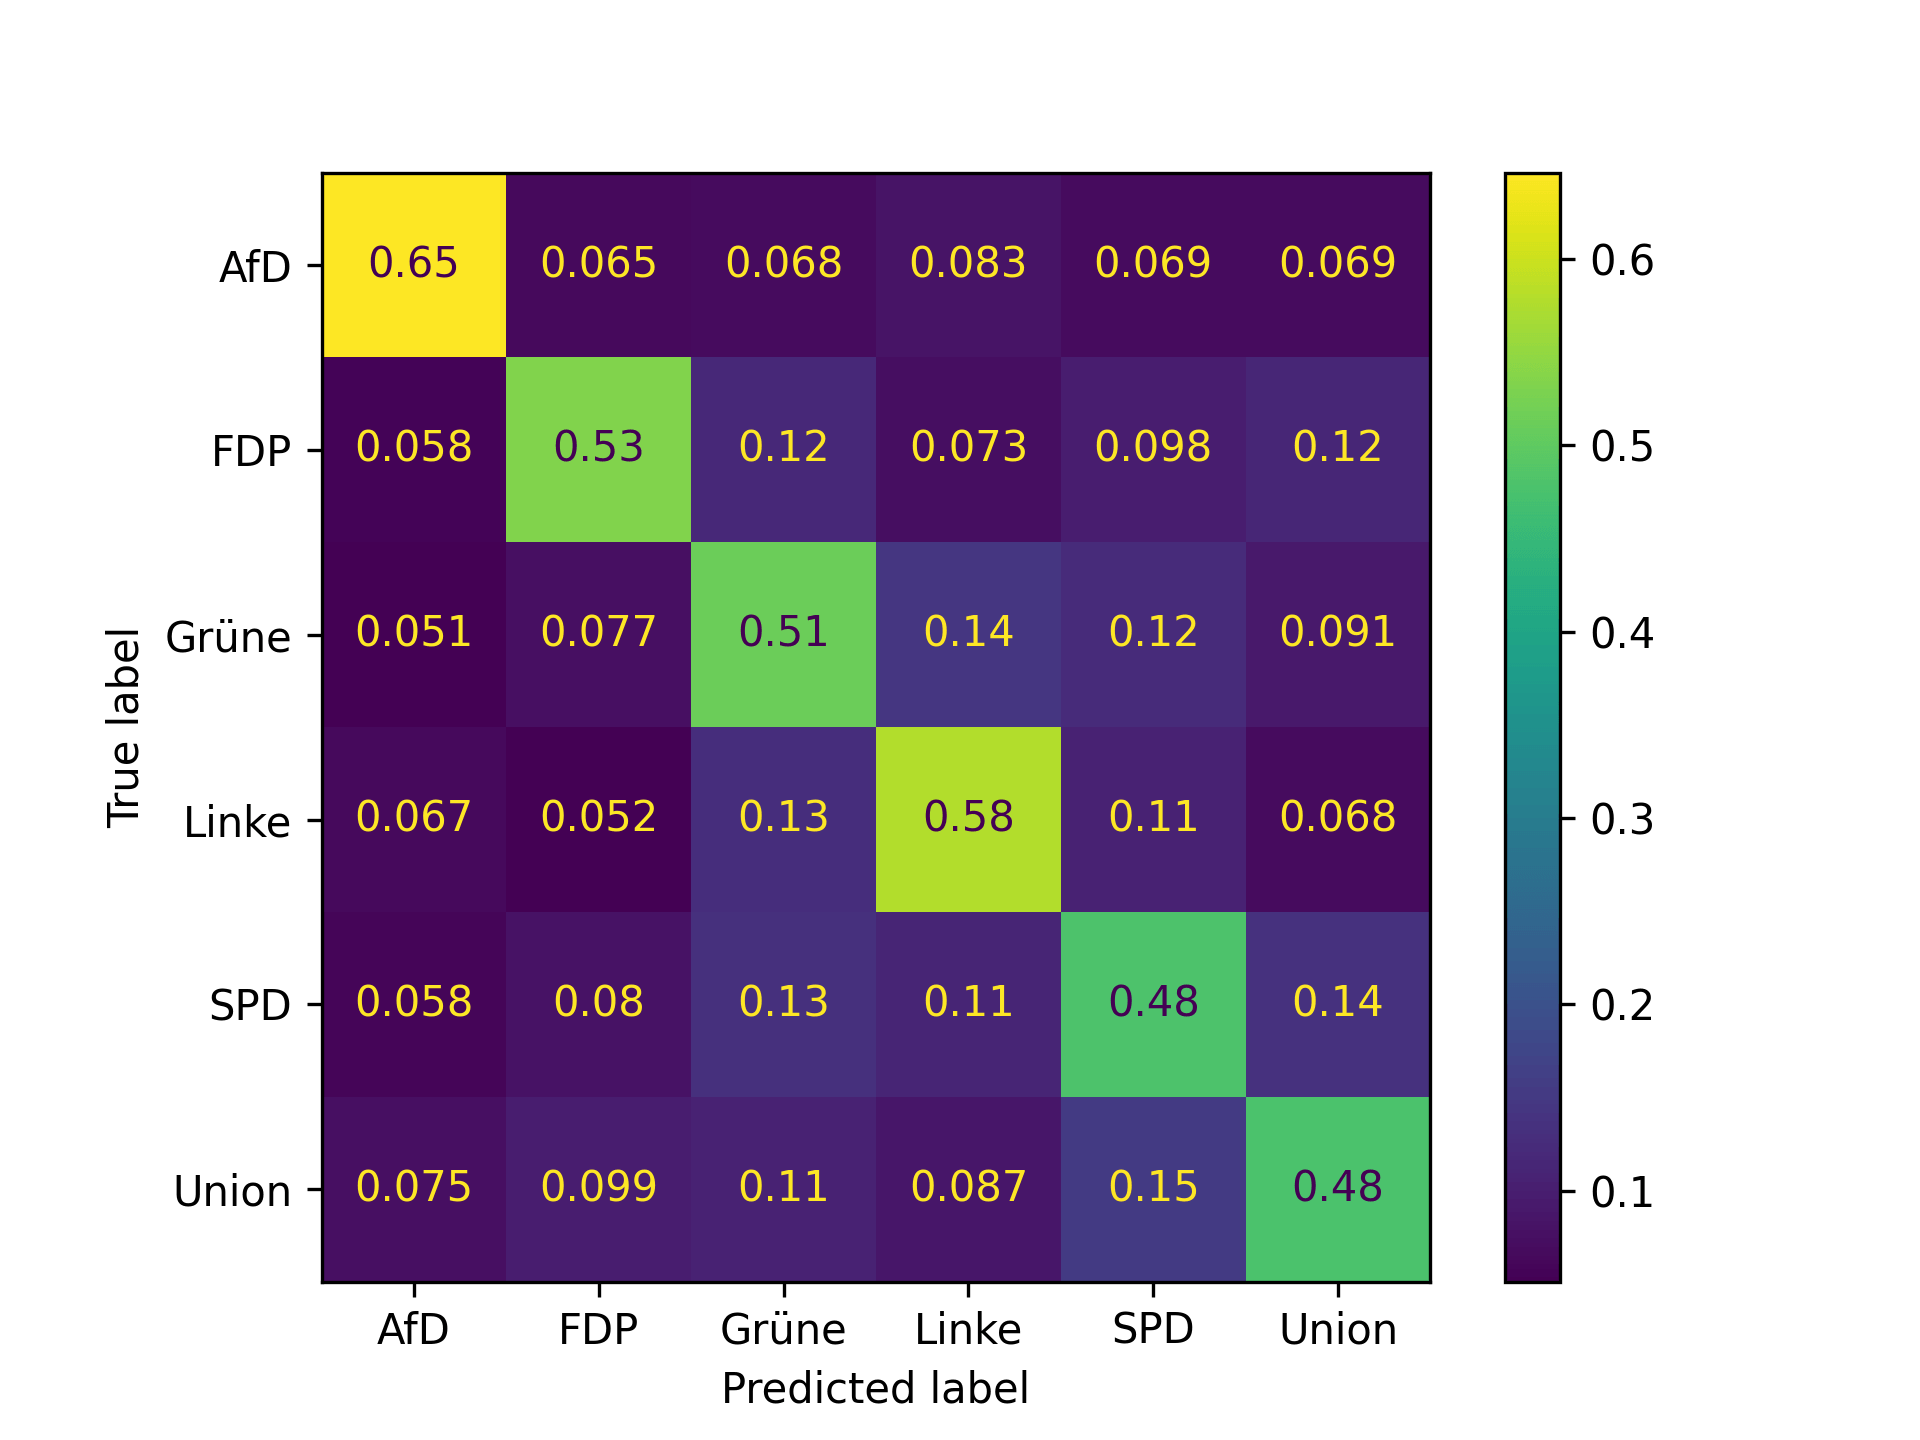
\includegraphics[width=0.9\textwidth]{data/images/modeling/baseline/none/tweets_confusion_matrix.png}
      \caption{Tweets (unbalanciert, \(N=\num{125000})\)} \label{sfig:confusionMatrixBaselineTweets}
    \end{subfigure}
    \begin{subfigure}{0.5\textwidth}
      \centering
      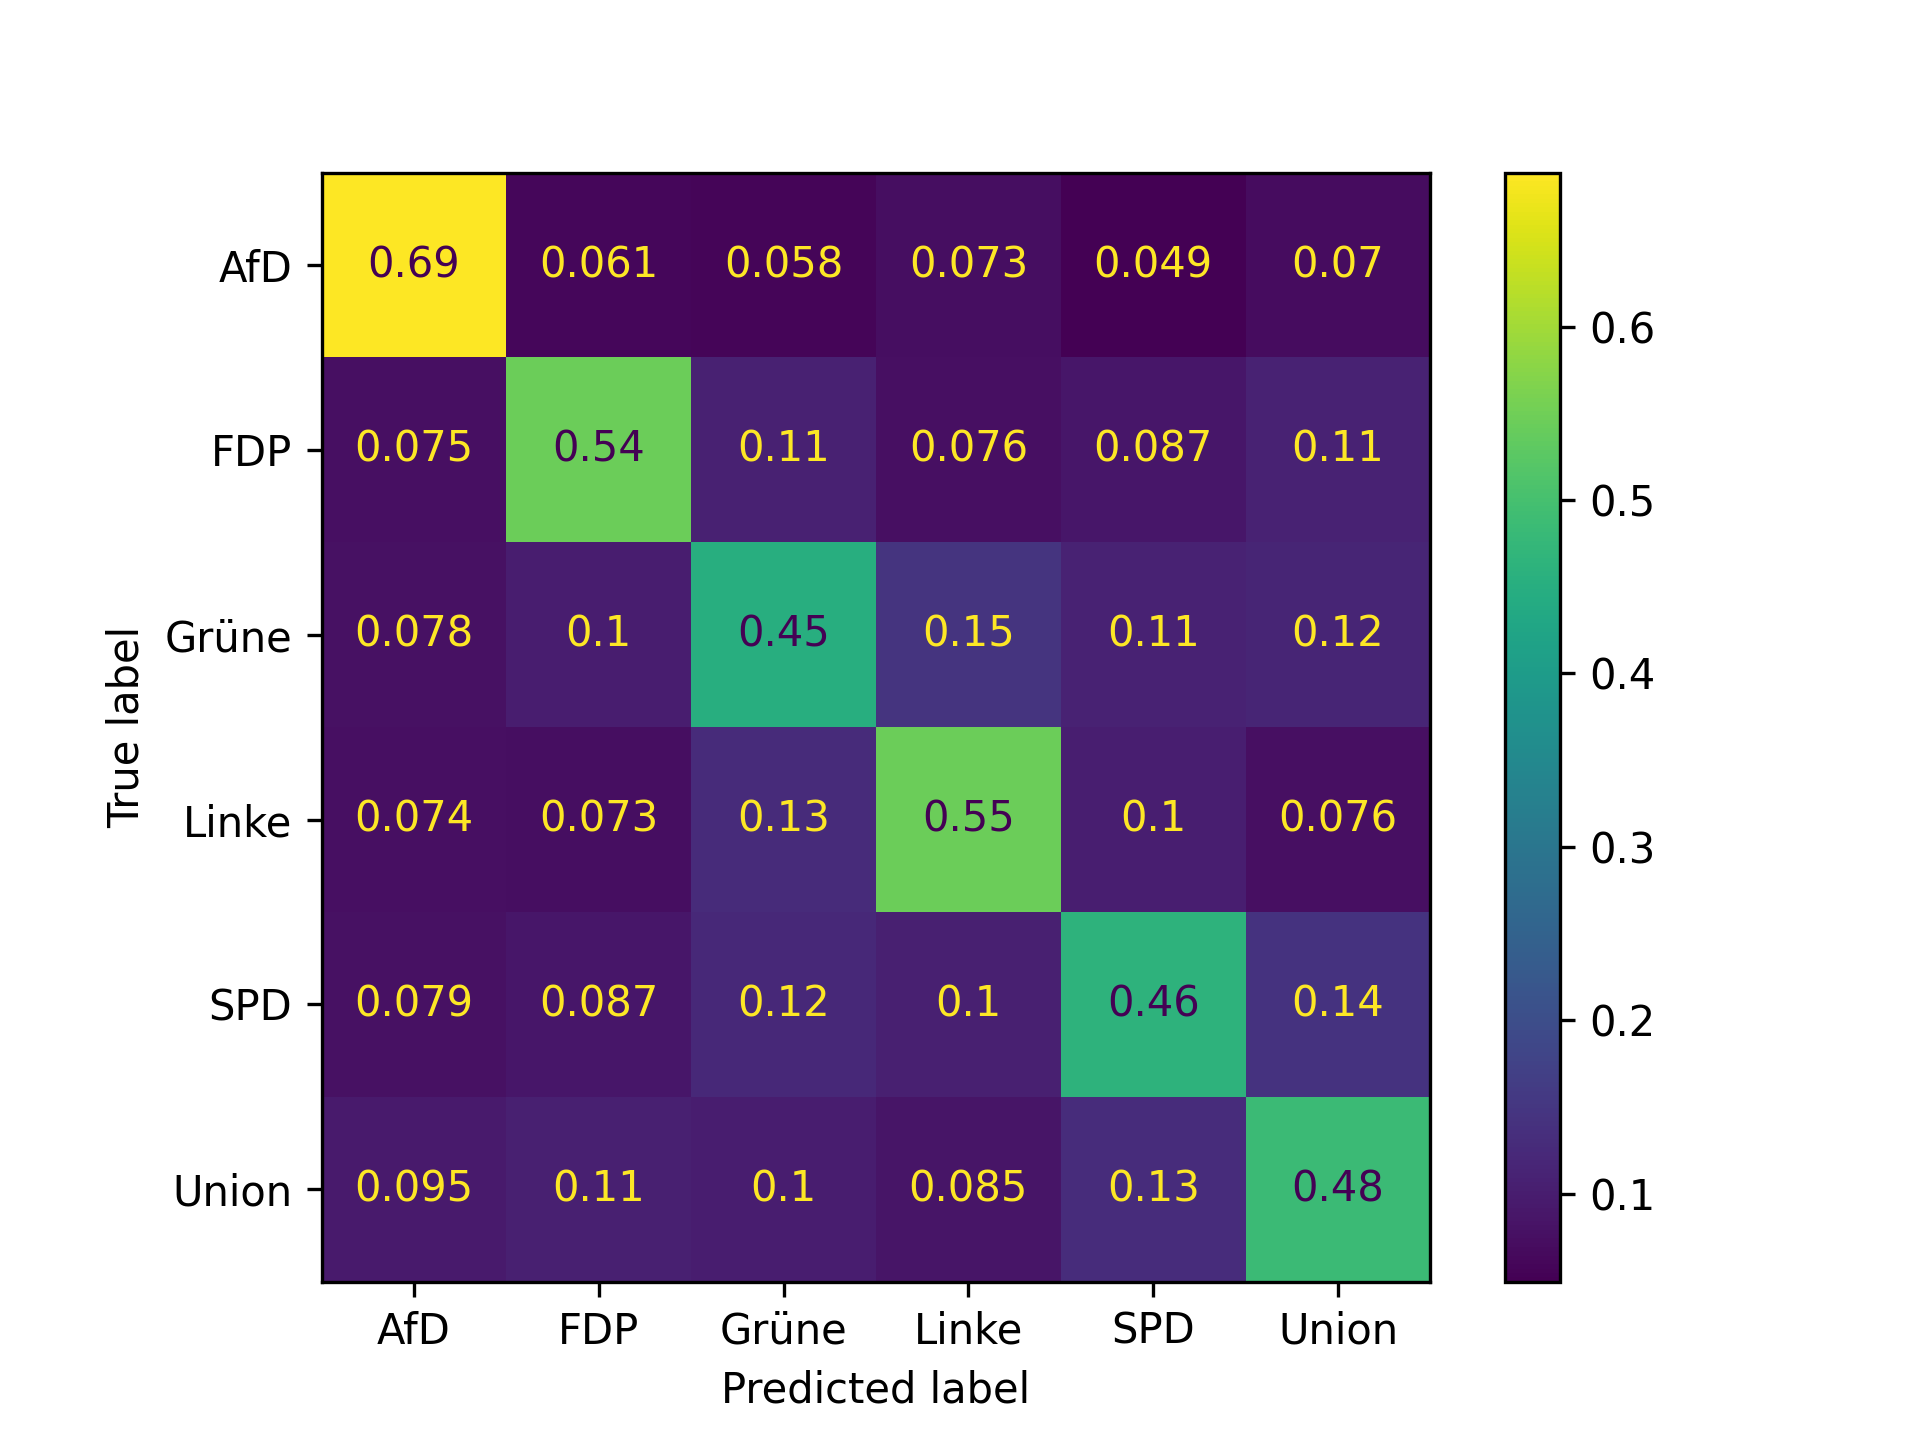
\includegraphics[width=0.9\textwidth]{data/images/modeling/baseline/under/tweets_confusion_matrix.png}
      \caption{Tweets (balanciert, \(N=\num{97906})\)} \label{sfig:confusionMatrixBaselineTweetsBalanced}
    \end{subfigure}
    
    \begin{subfigure}{0.5\textwidth}
      \centering
      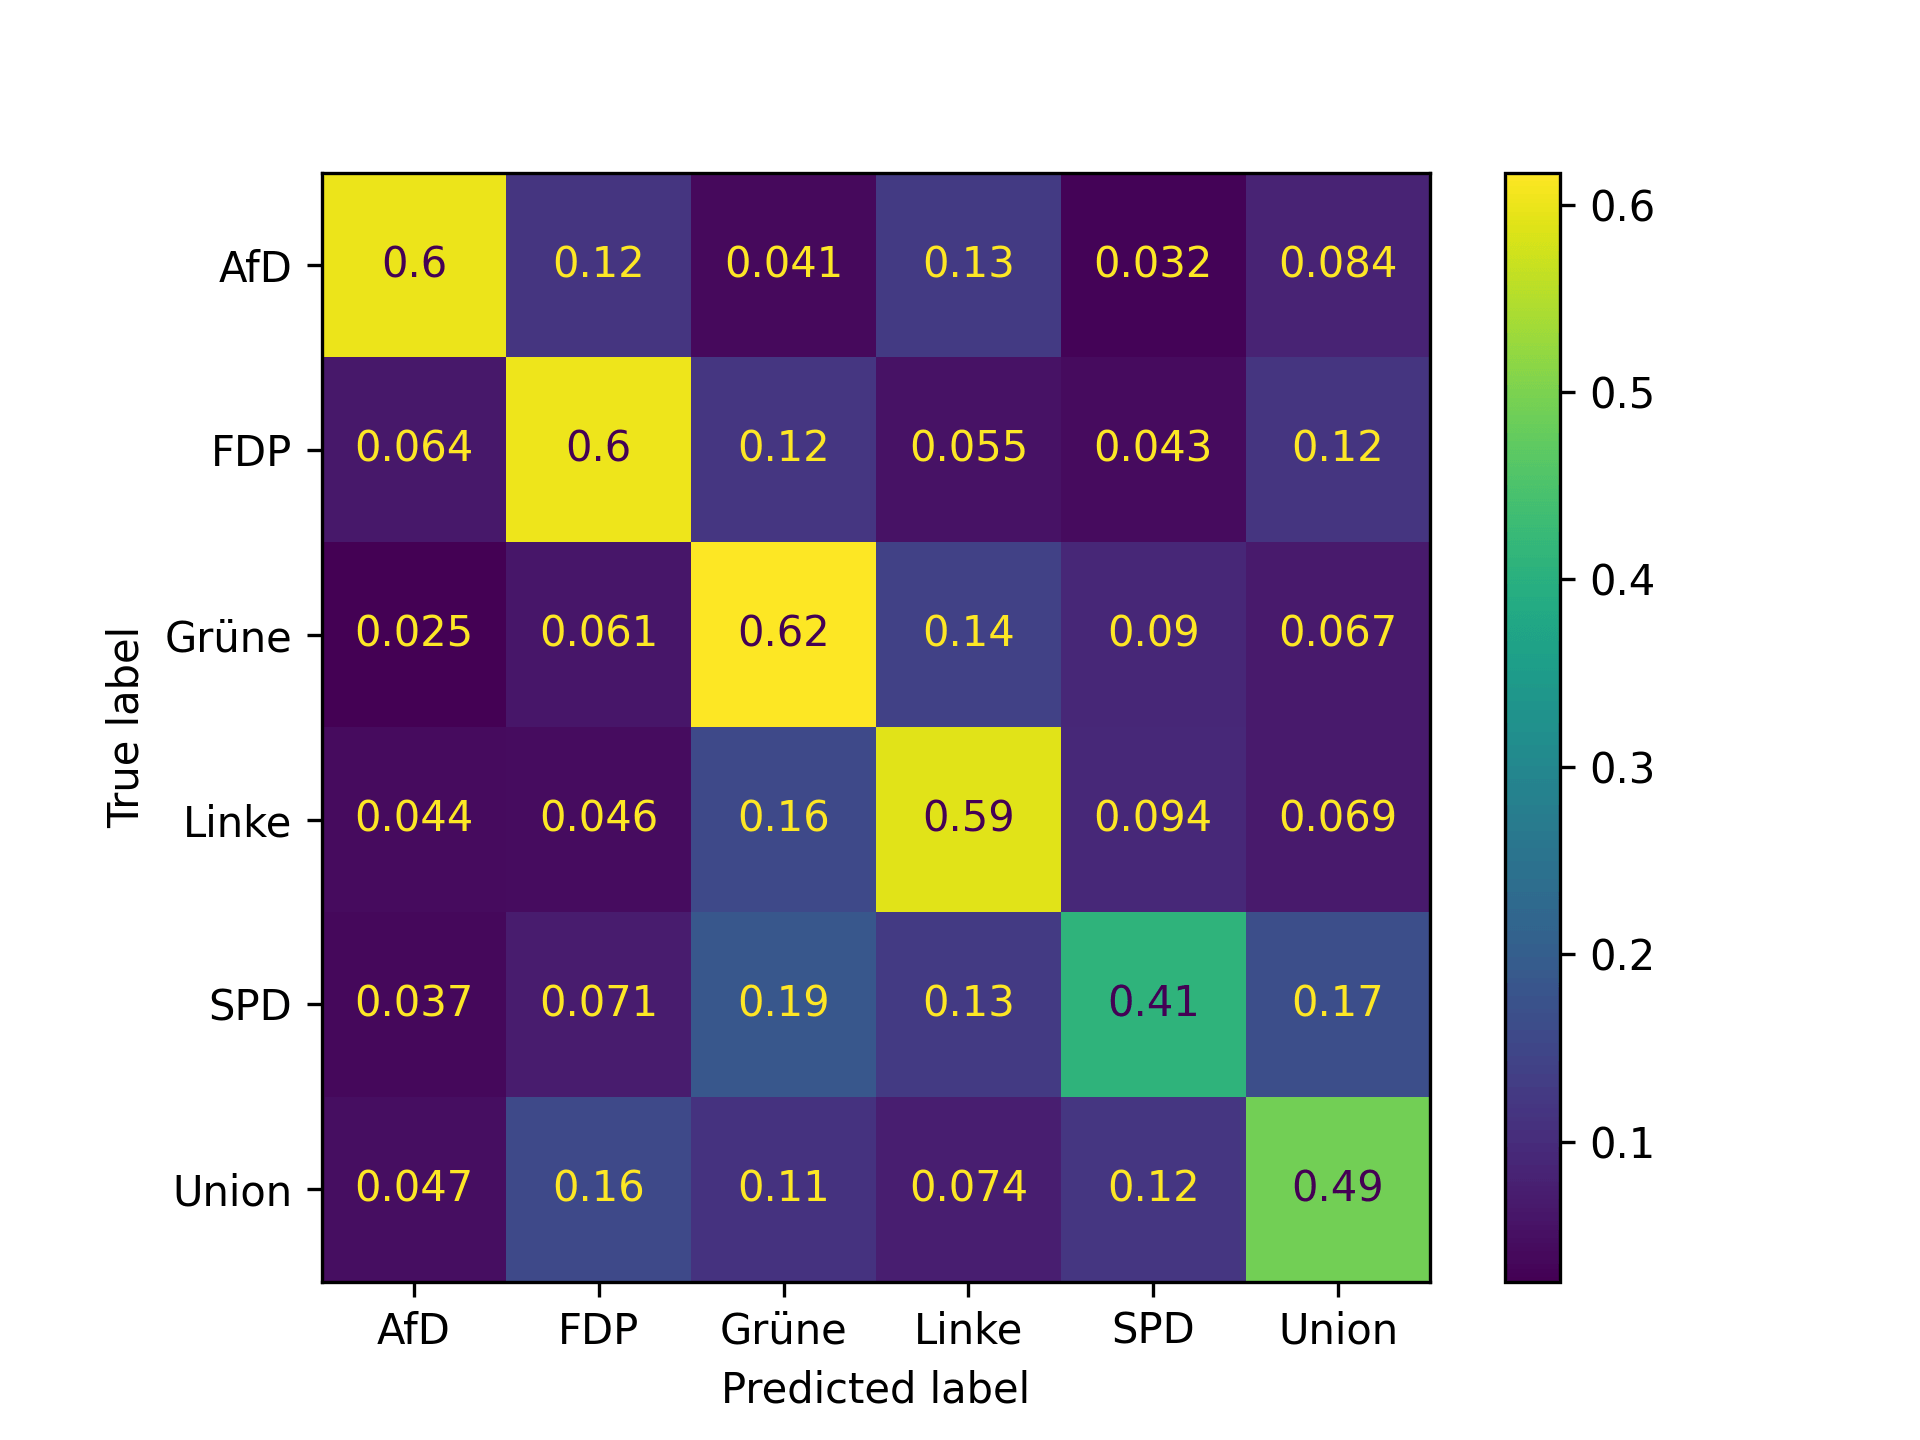
\includegraphics[width=0.9\textwidth]{data/images/modeling/baseline/none/party_programs_confusion_matrix.png}
      \caption{Wahlprogramme (unbalanciert, \(N=\num{27674}\))} \label{sfig:confusionMatrixBaselineManifest}
    \end{subfigure}
    \begin{subfigure}{0.5\textwidth}
      \centering
      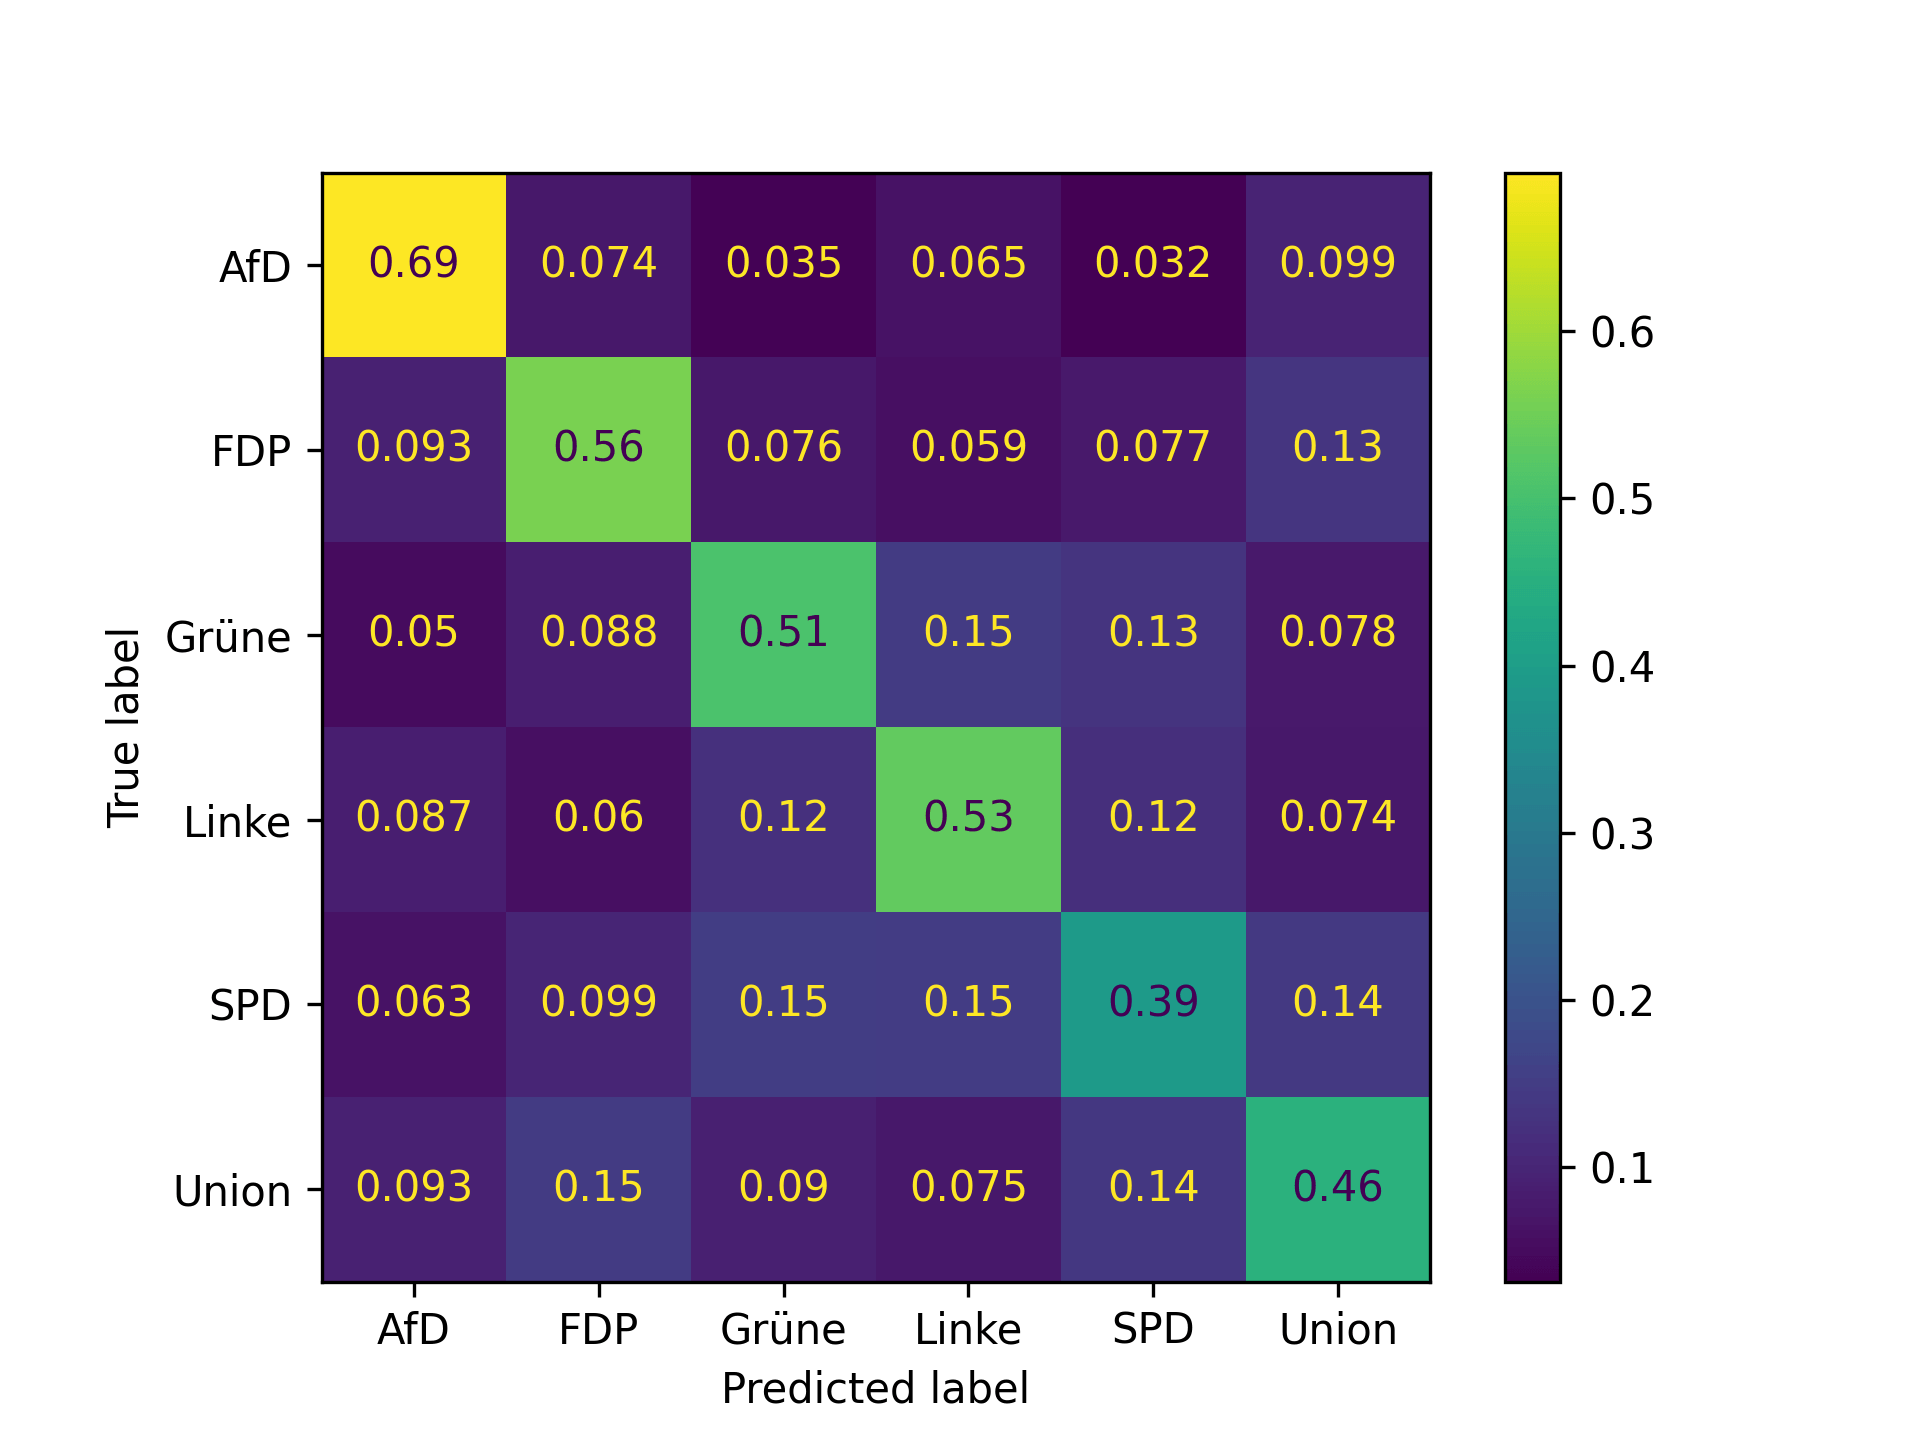
\includegraphics[width=0.9\textwidth]{data/images/modeling/baseline/under/party_programs_confusion_matrix.png}
      \caption{Wahlprogramme (balanciert, \(N=\num{18021})\)} \label{sfig:confusionMatrixBaselineManifestBalanced}
    \end{subfigure}
    
    \begin{subfigure}{0.5\textwidth}
      \centering
      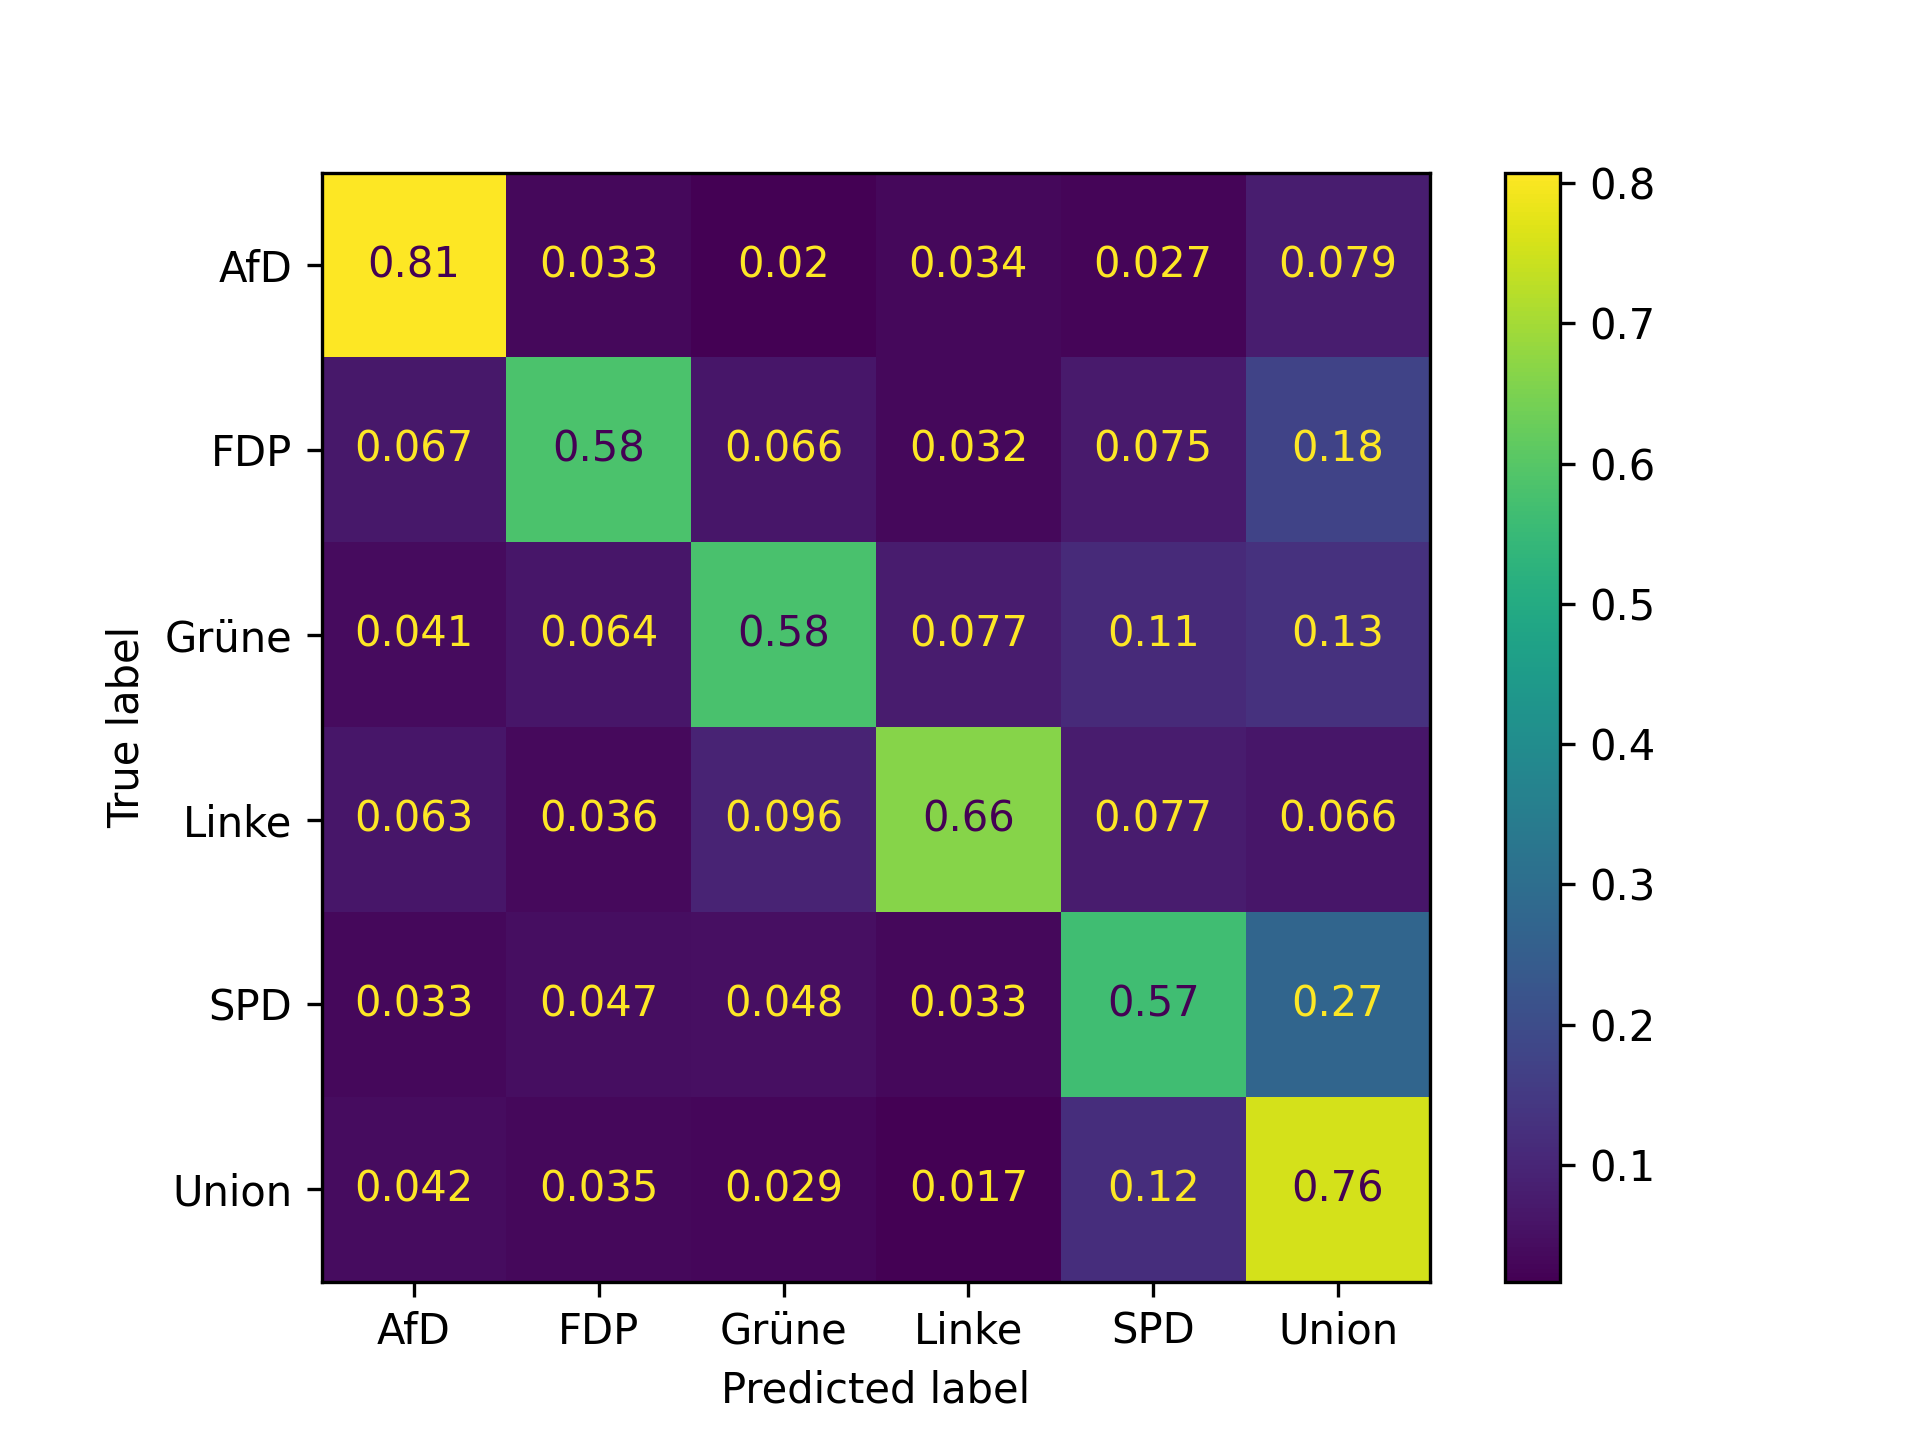
\includegraphics[width=0.9\textwidth]{data/images/modeling/baseline/none/speeches_confusion_matrix.png}
      \caption{Reden (unbalanciert, \(N=\num{38475})\)} \label{sfig:confusionMatrixBaselineSpeeches}
    \end{subfigure}
    \begin{subfigure}{0.5\textwidth}
      \centering
      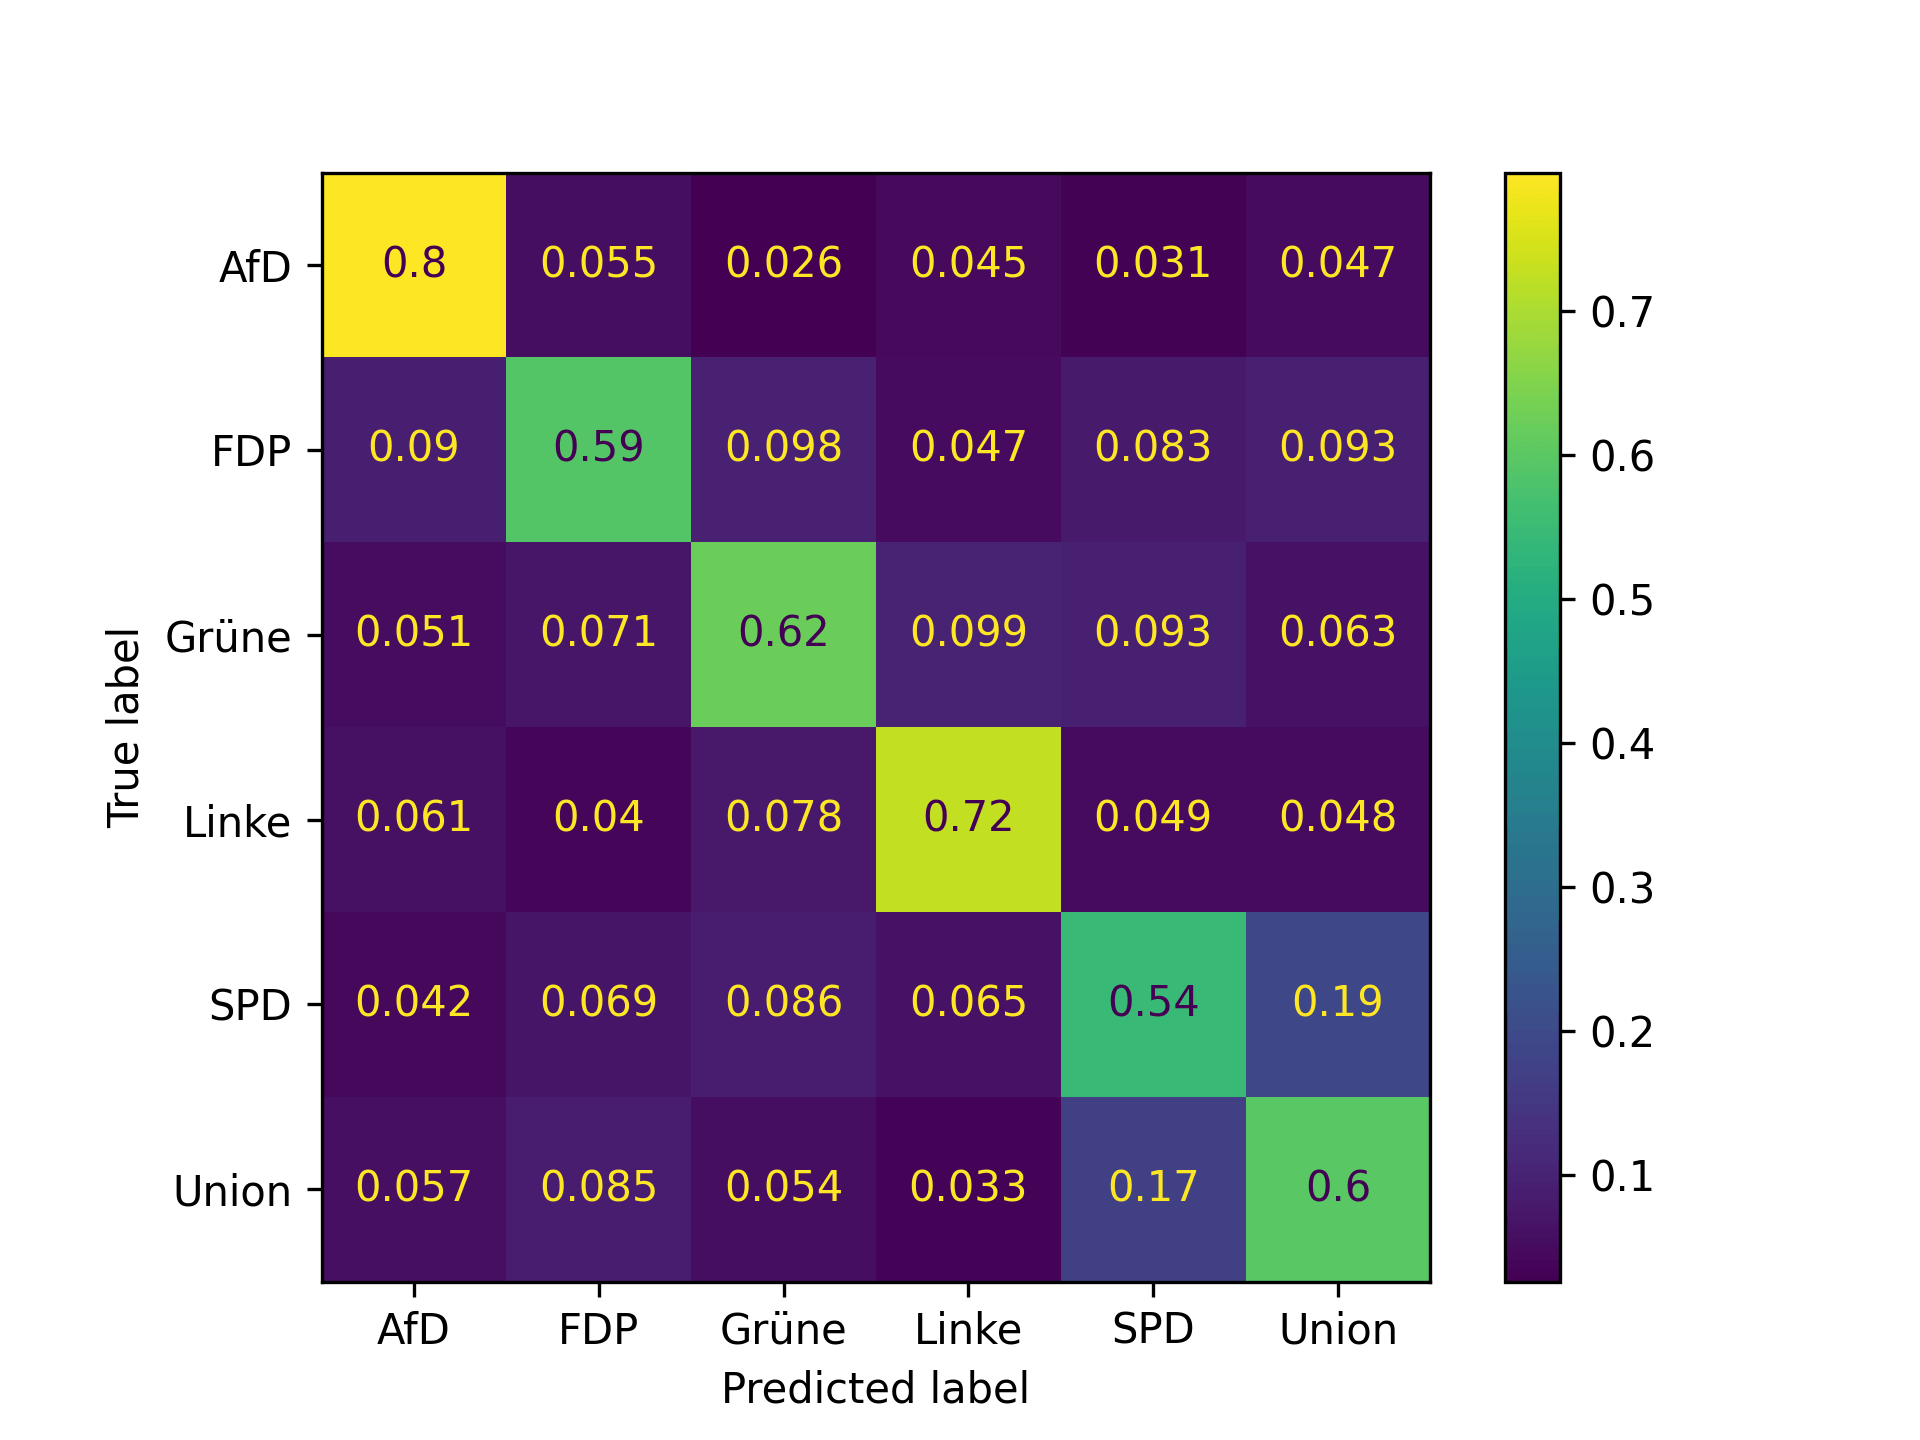
\includegraphics[width=0.9\textwidth]{data/images/modeling/baseline/under/speeches_confusion_matrix.png}
      \caption{Reden (balanciert, \(N=\num{28341})\)} \label{sfig:confusionMatrixBaselineSpeechesBalanced}
    \end{subfigure}
    
    \caption[Konfusionsmatritzen für Multinomial \acs{NB} und \acs{TF-IDF} auf unausgeglichen und ausgeglichenen Datensätzen]{Konfusionsmatritzen für Multinomial \acs{NB} und \acs{TF-IDF} auf unausgeglichen und ausgeglichenen Datensätzen. $N$ repräsentiert die Anzahl an Trainings- und Testdaten.} \label{fig:confusionMatrixBaseline}
\end{figure}

\subsection{fastText}

\ft ist eine Methode zum Generieren von Worteinbettungen, die von Facebook Research entwickelt wird \autocite{joulin_bag_2016}. Wie schon in \autoref{sec:representationForms} dargelegt, basiert die Methodik darauf, Wörter in n-grams zu zerlegen. Resultierend lassen sich ebenfalls Wörter klassifizieren, welche nicht im Trainingsdatensatz für die Worteinbettungen enthalten waren. Auf den sich ergebenen Worteinbettungen kann schließlich ein Klassifikator trainiert werden.

Für das folgende Training wird die \href{https://pypi.org/project/fasttext/}{\ft} Bibliothek für Python verwendet. Um die Worteinbettungen von \ft zu nutzen ist es möglich entweder eigenständig die Einbettungen zu trainieren, oder vortrainierte Einbettungen zu verwenden. Im Rahmen dieser Arbeit verwenden wir \href{https://fasttext.cc/docs/en/crawl-vectors.html}{vortrainierte Einbettungen}, da die Erstellung solcher Einbettungen eine große Menge an Daten benötigt. Die deutschen, vortrainierten Worteinbettungen basieren auf dem \href{https://commoncrawl.org/}{Common Crawl} und \href{https://www.wikipedia.org/}{Wikipedia} Datensatz.

Das Training erfolgt auf allen Einträgen pro Datensatz für jeweils \num{5} Epochen. Die Lernrate wird auf \num{0.1} angesetzt. Für das Training wird, ebenfalls wie bei \textcite{guhr_training_2020}, Bigramme verwendet. Zusätzlich werden andere Längen getestet, um zu prüfen, ob und welchen Effekt diese bei den ausgewählten Datensätzen hat. Wie zuvor erwähnt werden die deutschen, vortrainierten Worteinbettungen, mit einer Vektorgröße von \num{300}, verwenden.

\begin{table}[H]
    \centering
    \caption{Makro \(F_1\) Score für Supervised Learning mittels \ft} \label{tab:overviewScoresFastText}
    {\footnotesize
    \begin{tblr}{width=\textwidth, hline{1-2, Z} = {1pt}, colspec={lQ[si={table-format=1},c]*{2}{Q[si={table-format=1.2},c]}}, row{1}={guard,font=\bfseries,l}}
        Datensatz & N-Grams & Unbalanced & Balanced \\ 

        Tweets & \SetCell[r=3]{c} 2 & 0.60 & 0.58 \\
        Wahlprogramm & & 0.57 & 0.54 \\
        Reden & & 0.58 & 0.56 \\
        \hline
        Tweets & \SetCell[r=3]{c} 3 & 0.59 & 0.57 \\
        Wahlprogramm & & 0.56 & 0.53 \\
        Reden & & 0.48 & 0.44 \\
    \end{tblr}
    }
\end{table}

\autoref{tab:overviewScoresFastText} zeigt, welche Ergebnisse sich mit \ft erreichen lassen. Das Training erfolgte mit Bigrammen und Trigrammen. Dabei wurde jeder Datensatz isoliert trainiert, um zunächst die Performance auf jeden Datensatz individuell zu testen. Aus den Ergebnissen geht hervor, dass durchweg das Training auf den unbalancierten Datensätzen zu höheren Makro \(F_1\) Scores geführt hat. Es zeigt sich, dass die meisten Trainings einen Score zwischen \numrange{0.53}{0.59} erreicht haben. Lediglich die unbalancierten Tweets mittels Bigrammen haben einen Score von \num{0.60} erreicht. Abgeschlagen finden sich die Reden mittels Trigrammen, welche lediglich einen \(F_1\) Score von \num{0.48} und \num{0.44} erreichten.

Bei näherer Betrachtung fällt auf, dass Trigramme konsequent zu einer Verschlechterung der Makro \(F_1\) Scores führt. Bei den Tweets und Wahlprogrammen handelt es sich zwar nur um einen Verlust von \num{0.01}, jedoch verliert der Score bei den Reden zwischen \num{0.1} und \num{0.12}.

% TODO: Alle Parameter beschreiben

\begin{figure}[H]
    \begin{subfigure}{0.5\textwidth}
      \centering
      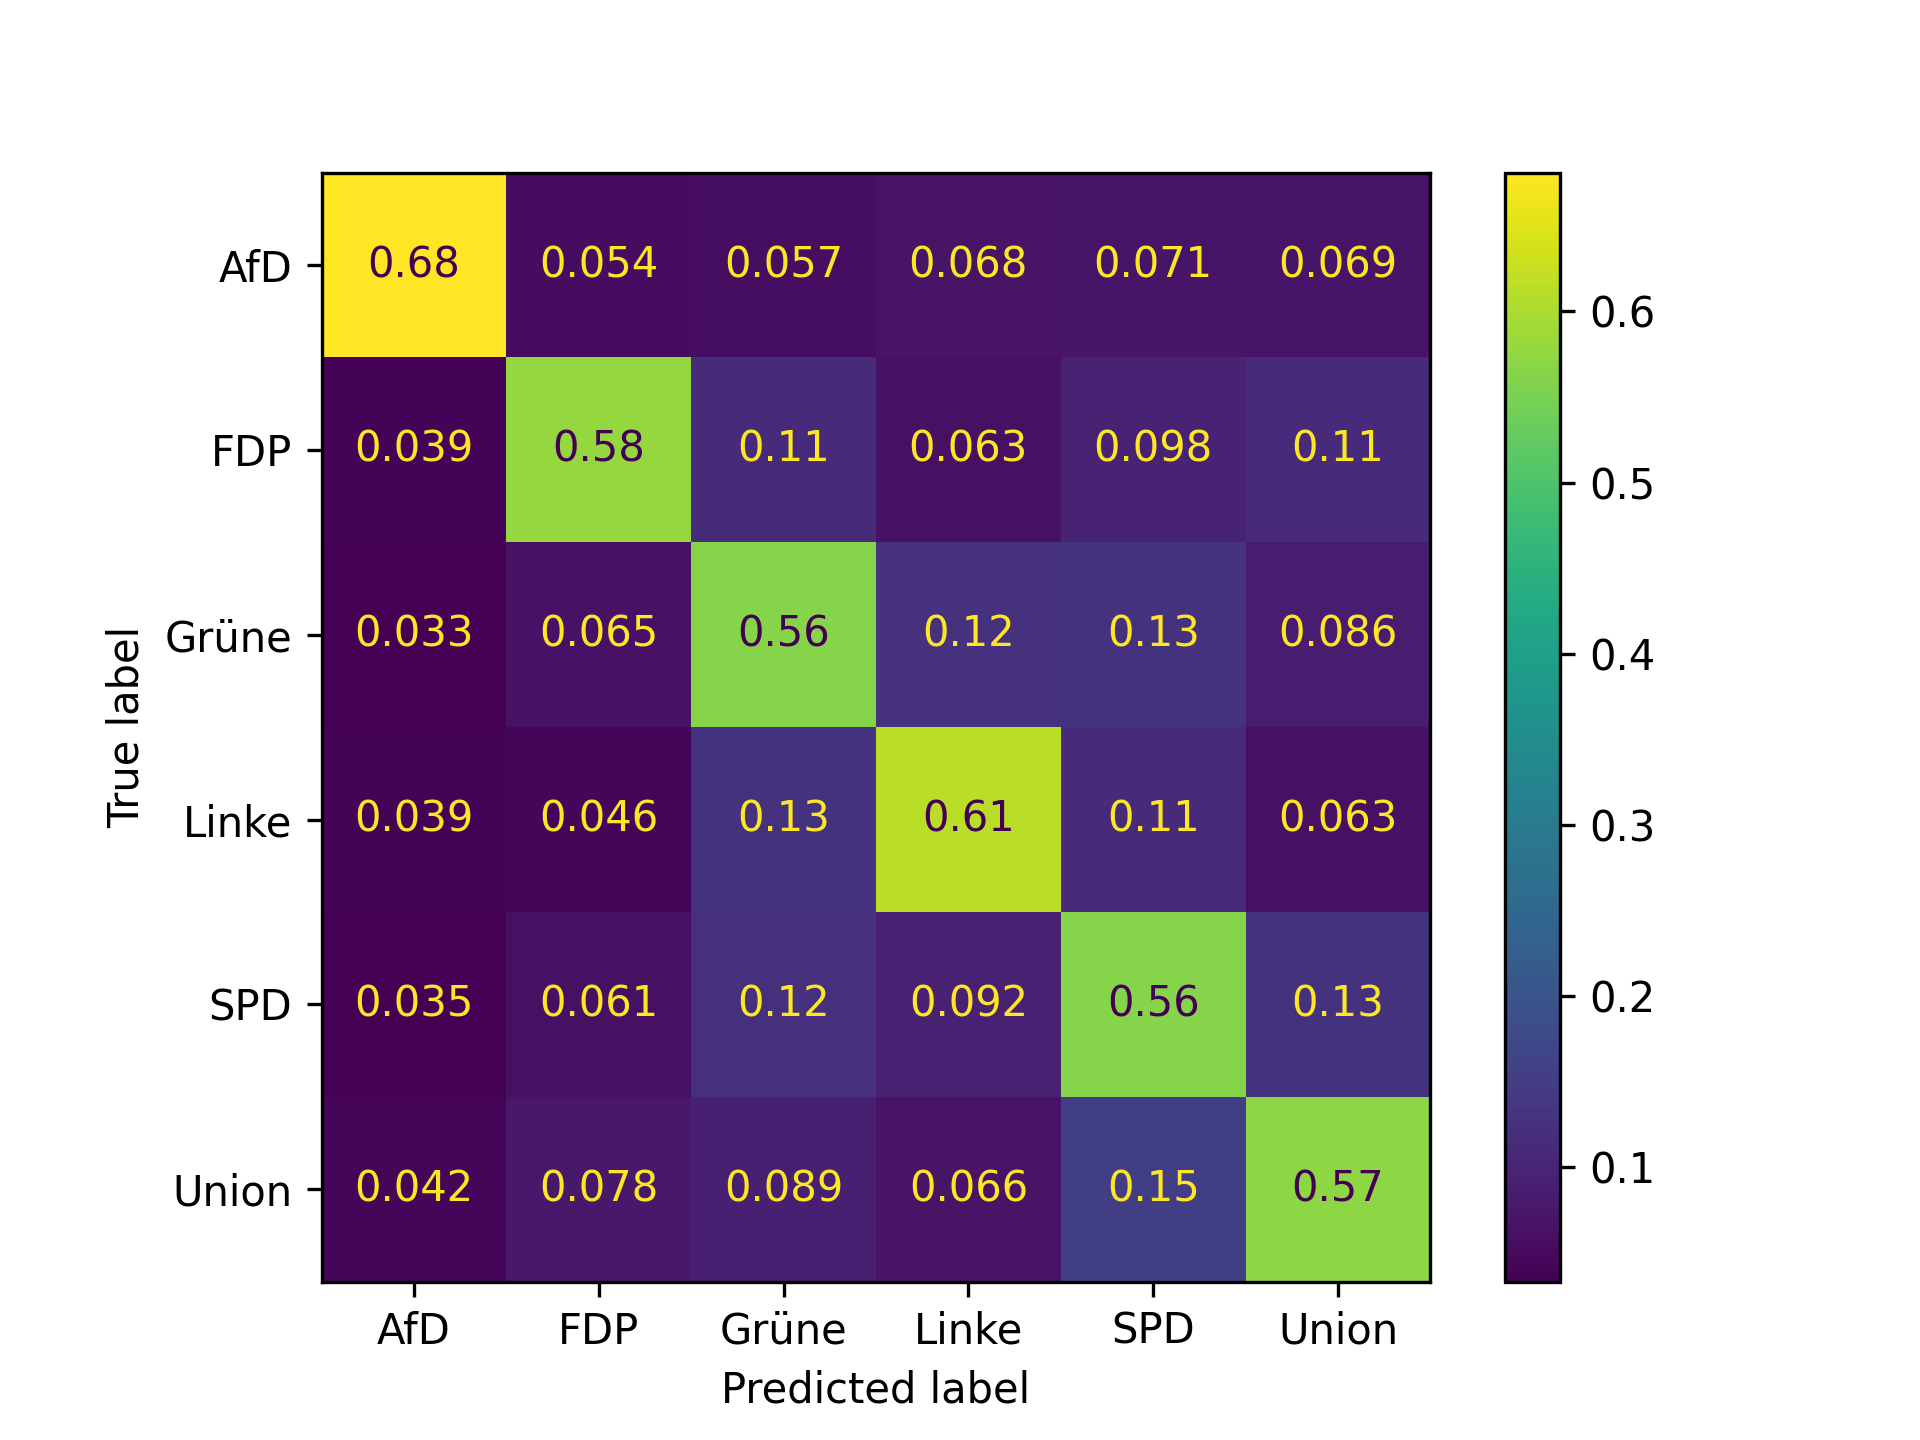
\includegraphics[width=0.9\textwidth]{data/images/modeling/fasttext/none/tweets_confusion_matrix.png}
      \caption{Tweets (unbalanciert, \(N = \num{326625}\))} \label{sfig:confusionMatrixFastTextTweets}
    \end{subfigure}
    \begin{subfigure}{0.5\textwidth}
      \centering
      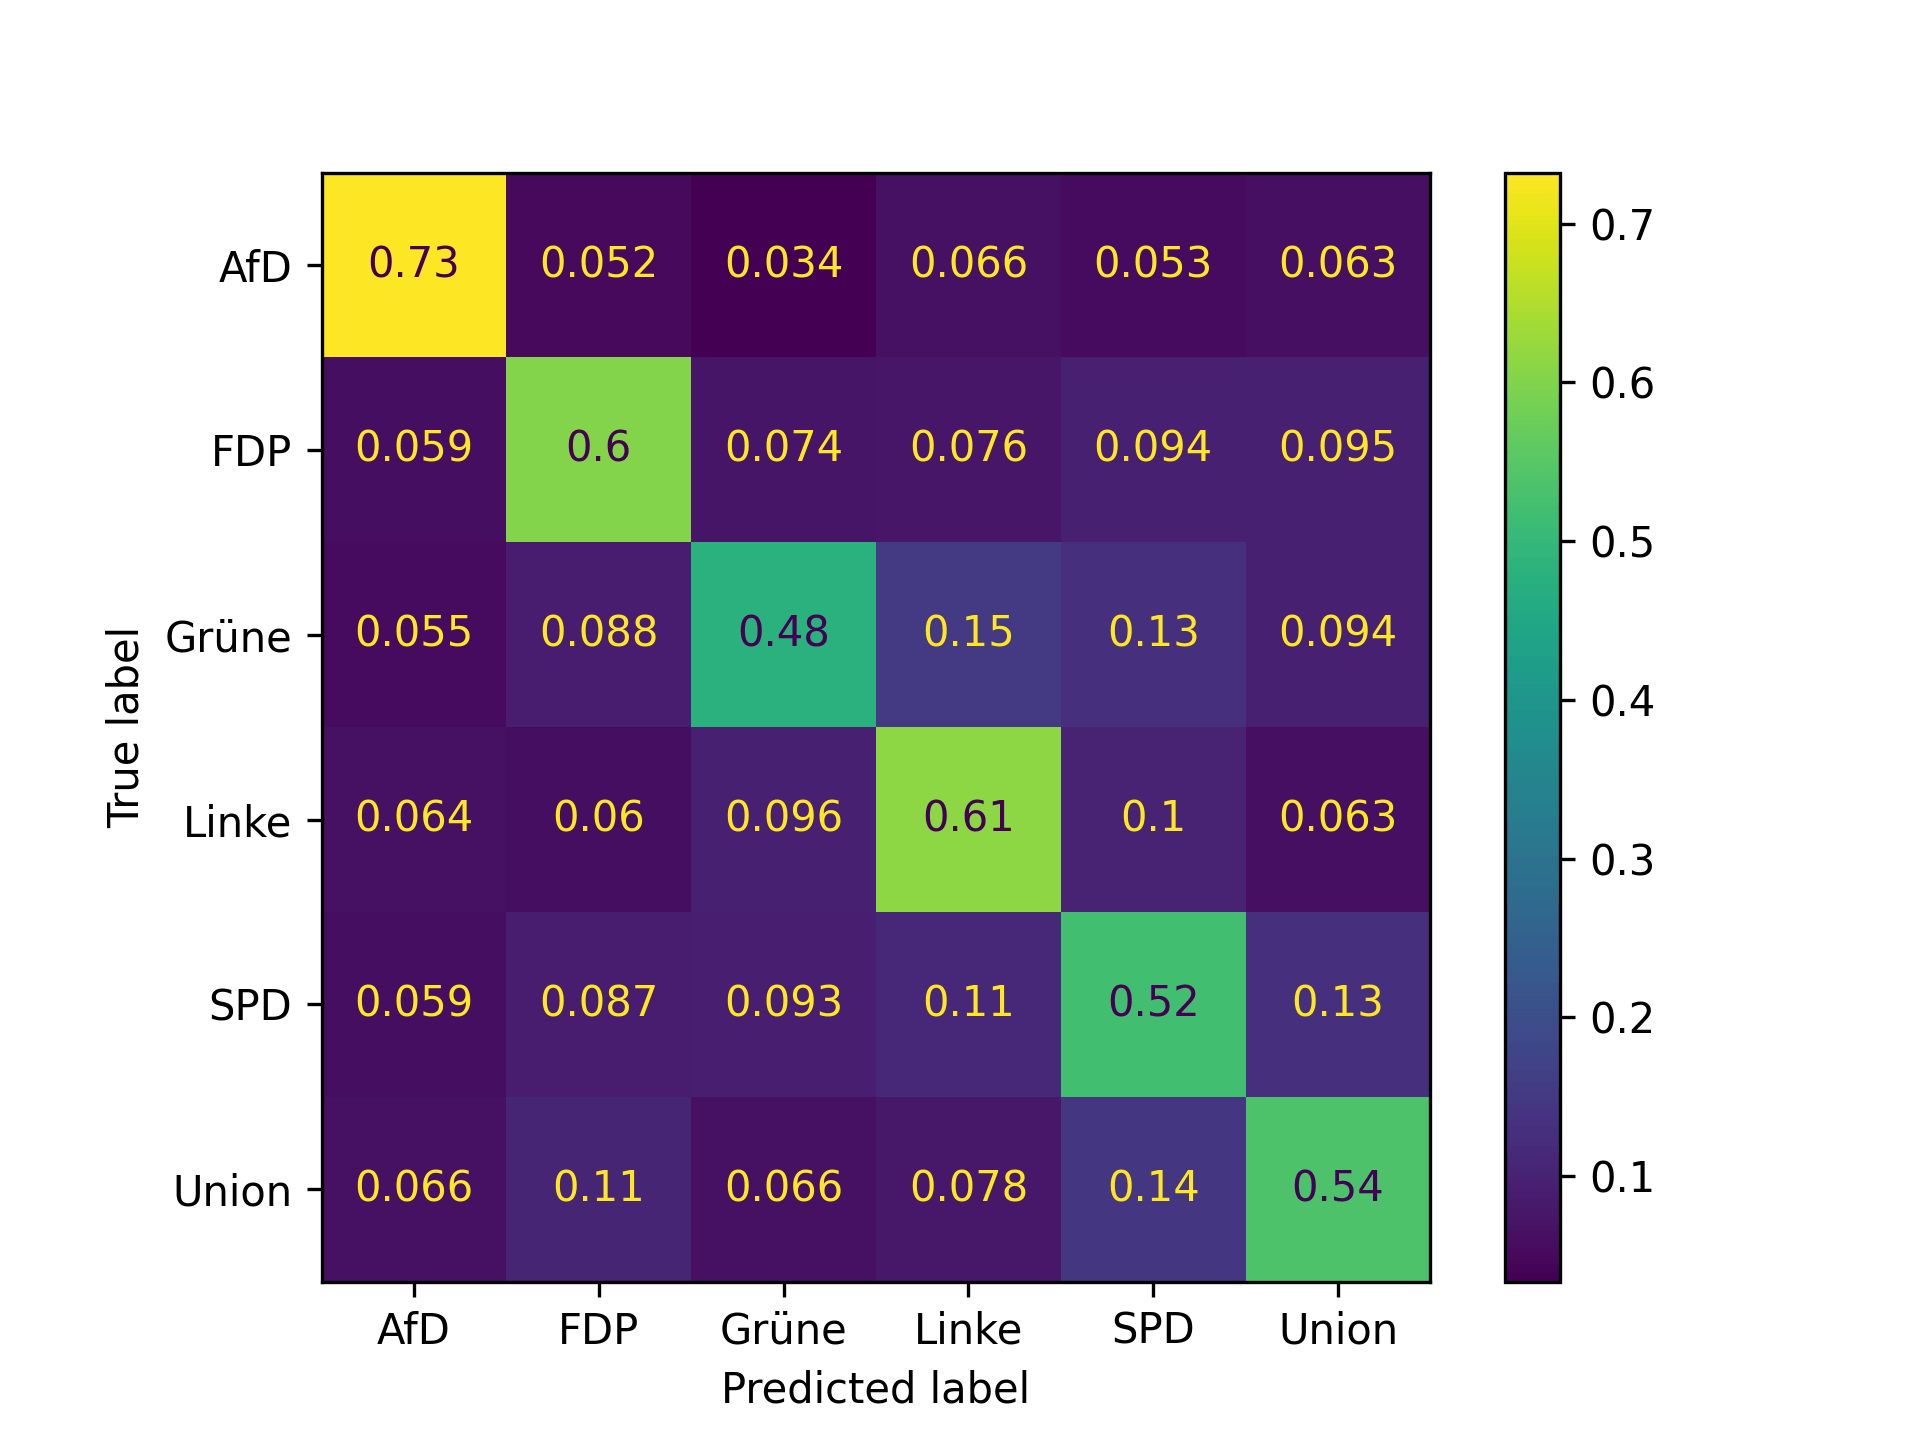
\includegraphics[width=0.9\textwidth]{data/images/modeling/fasttext/under/tweets_confusion_matrix.png}
      \caption{Tweets (balanciert, \(N = \num{255813}\))} \label{sfig:confusionMatrixFastTextTweetsBalanced}
    \end{subfigure}
    
    \begin{subfigure}{0.5\textwidth}
      \centering
      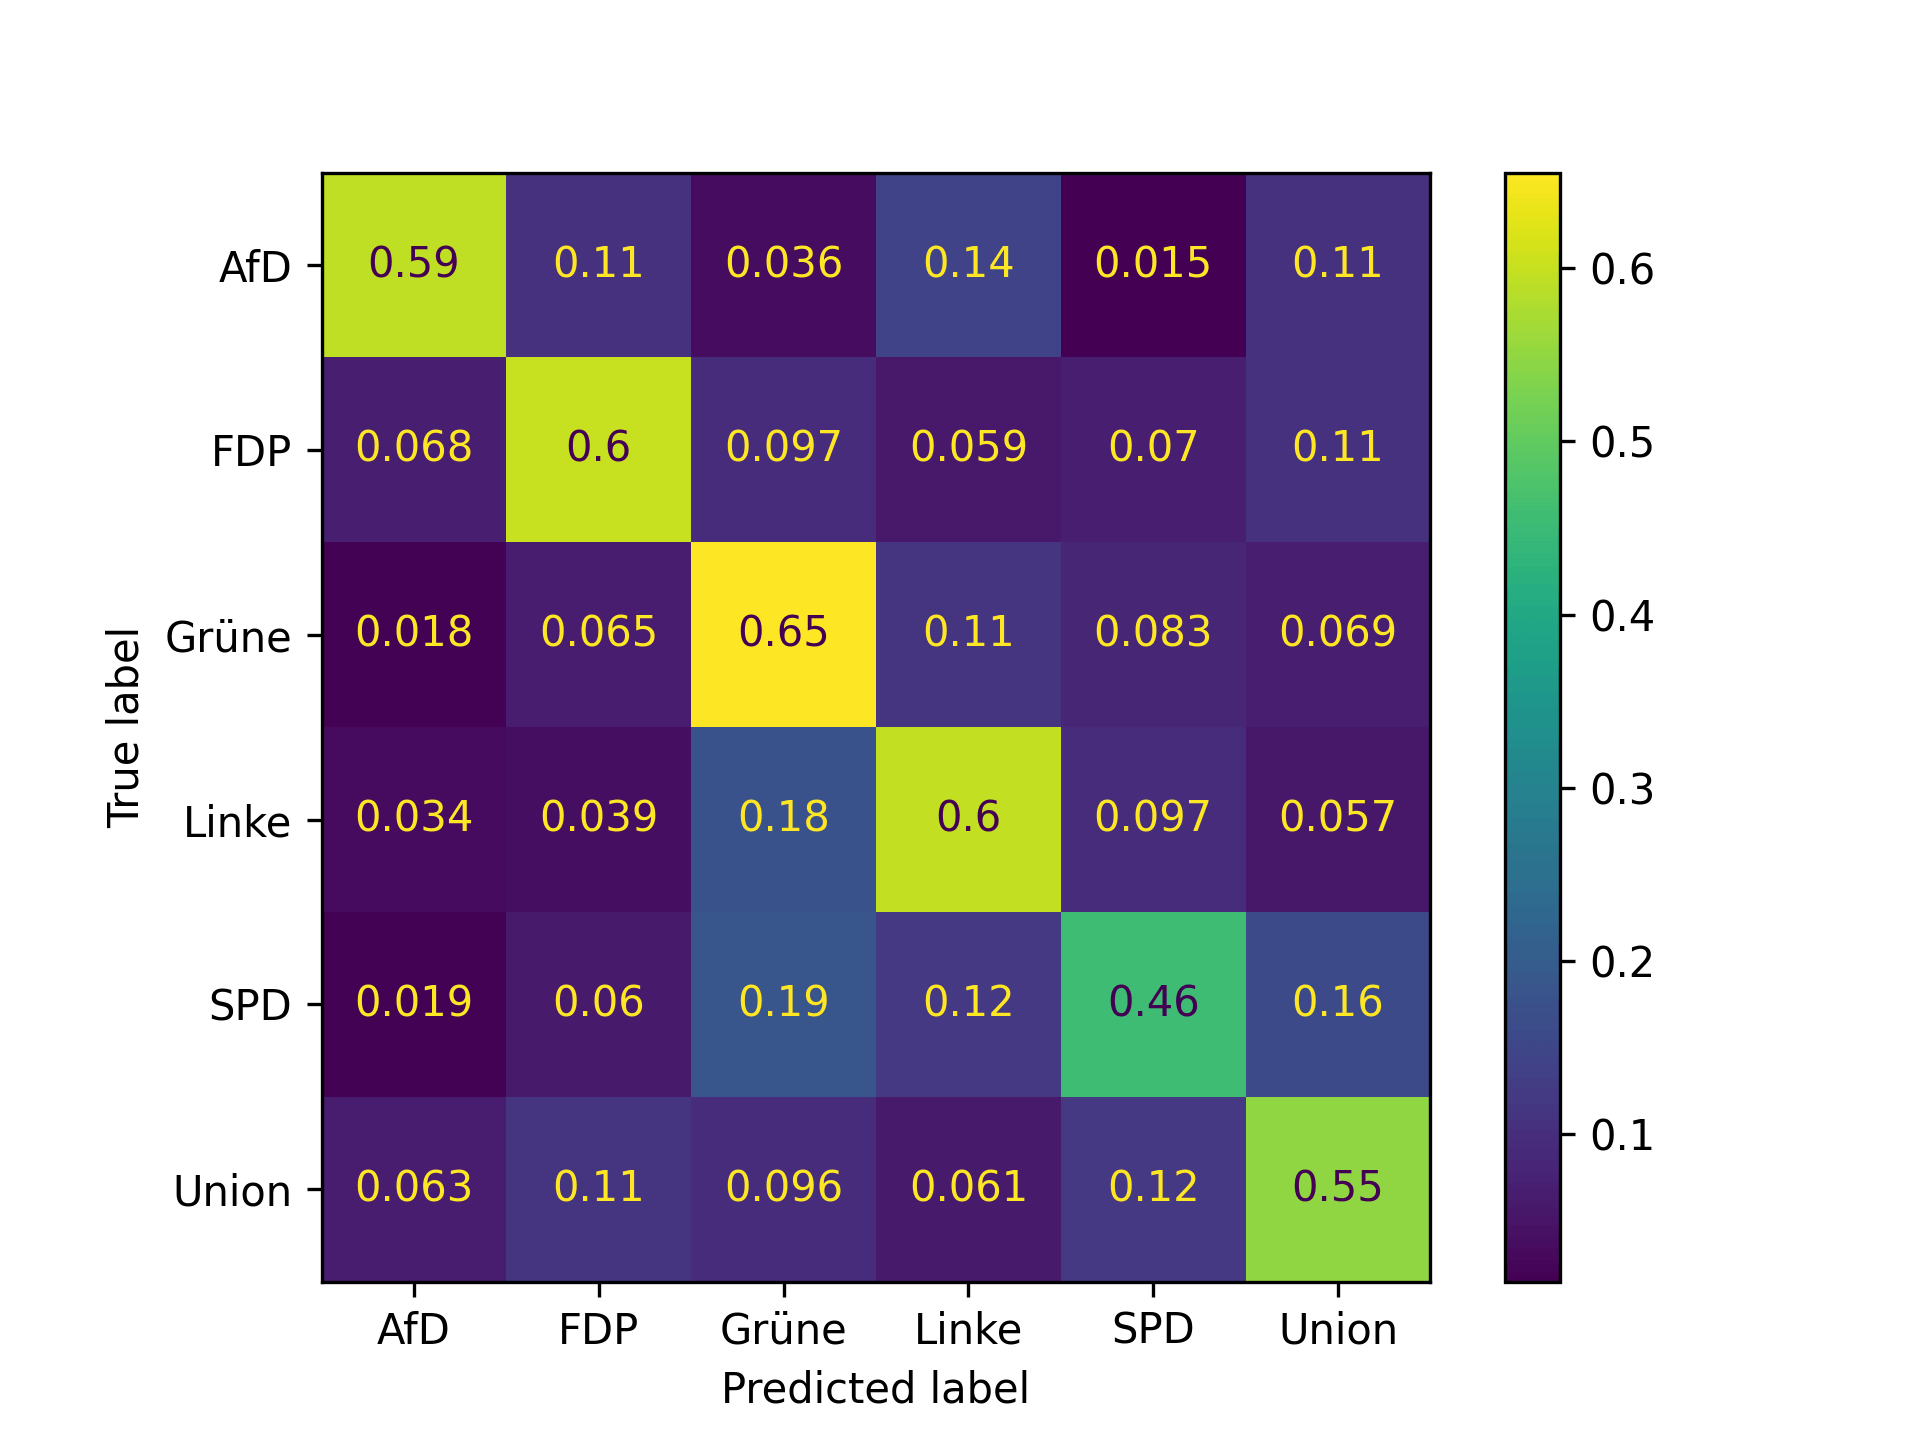
\includegraphics[width=0.9\textwidth]{data/images/modeling/fasttext/none/party_programs_confusion_matrix.png}
      \caption{Wahlprogramme (unbalanciert, \(N = \num{27674}\))} \label{sfig:confusionMatrixFastTextManifest}
    \end{subfigure}
    \begin{subfigure}{0.5\textwidth}
      \centering
      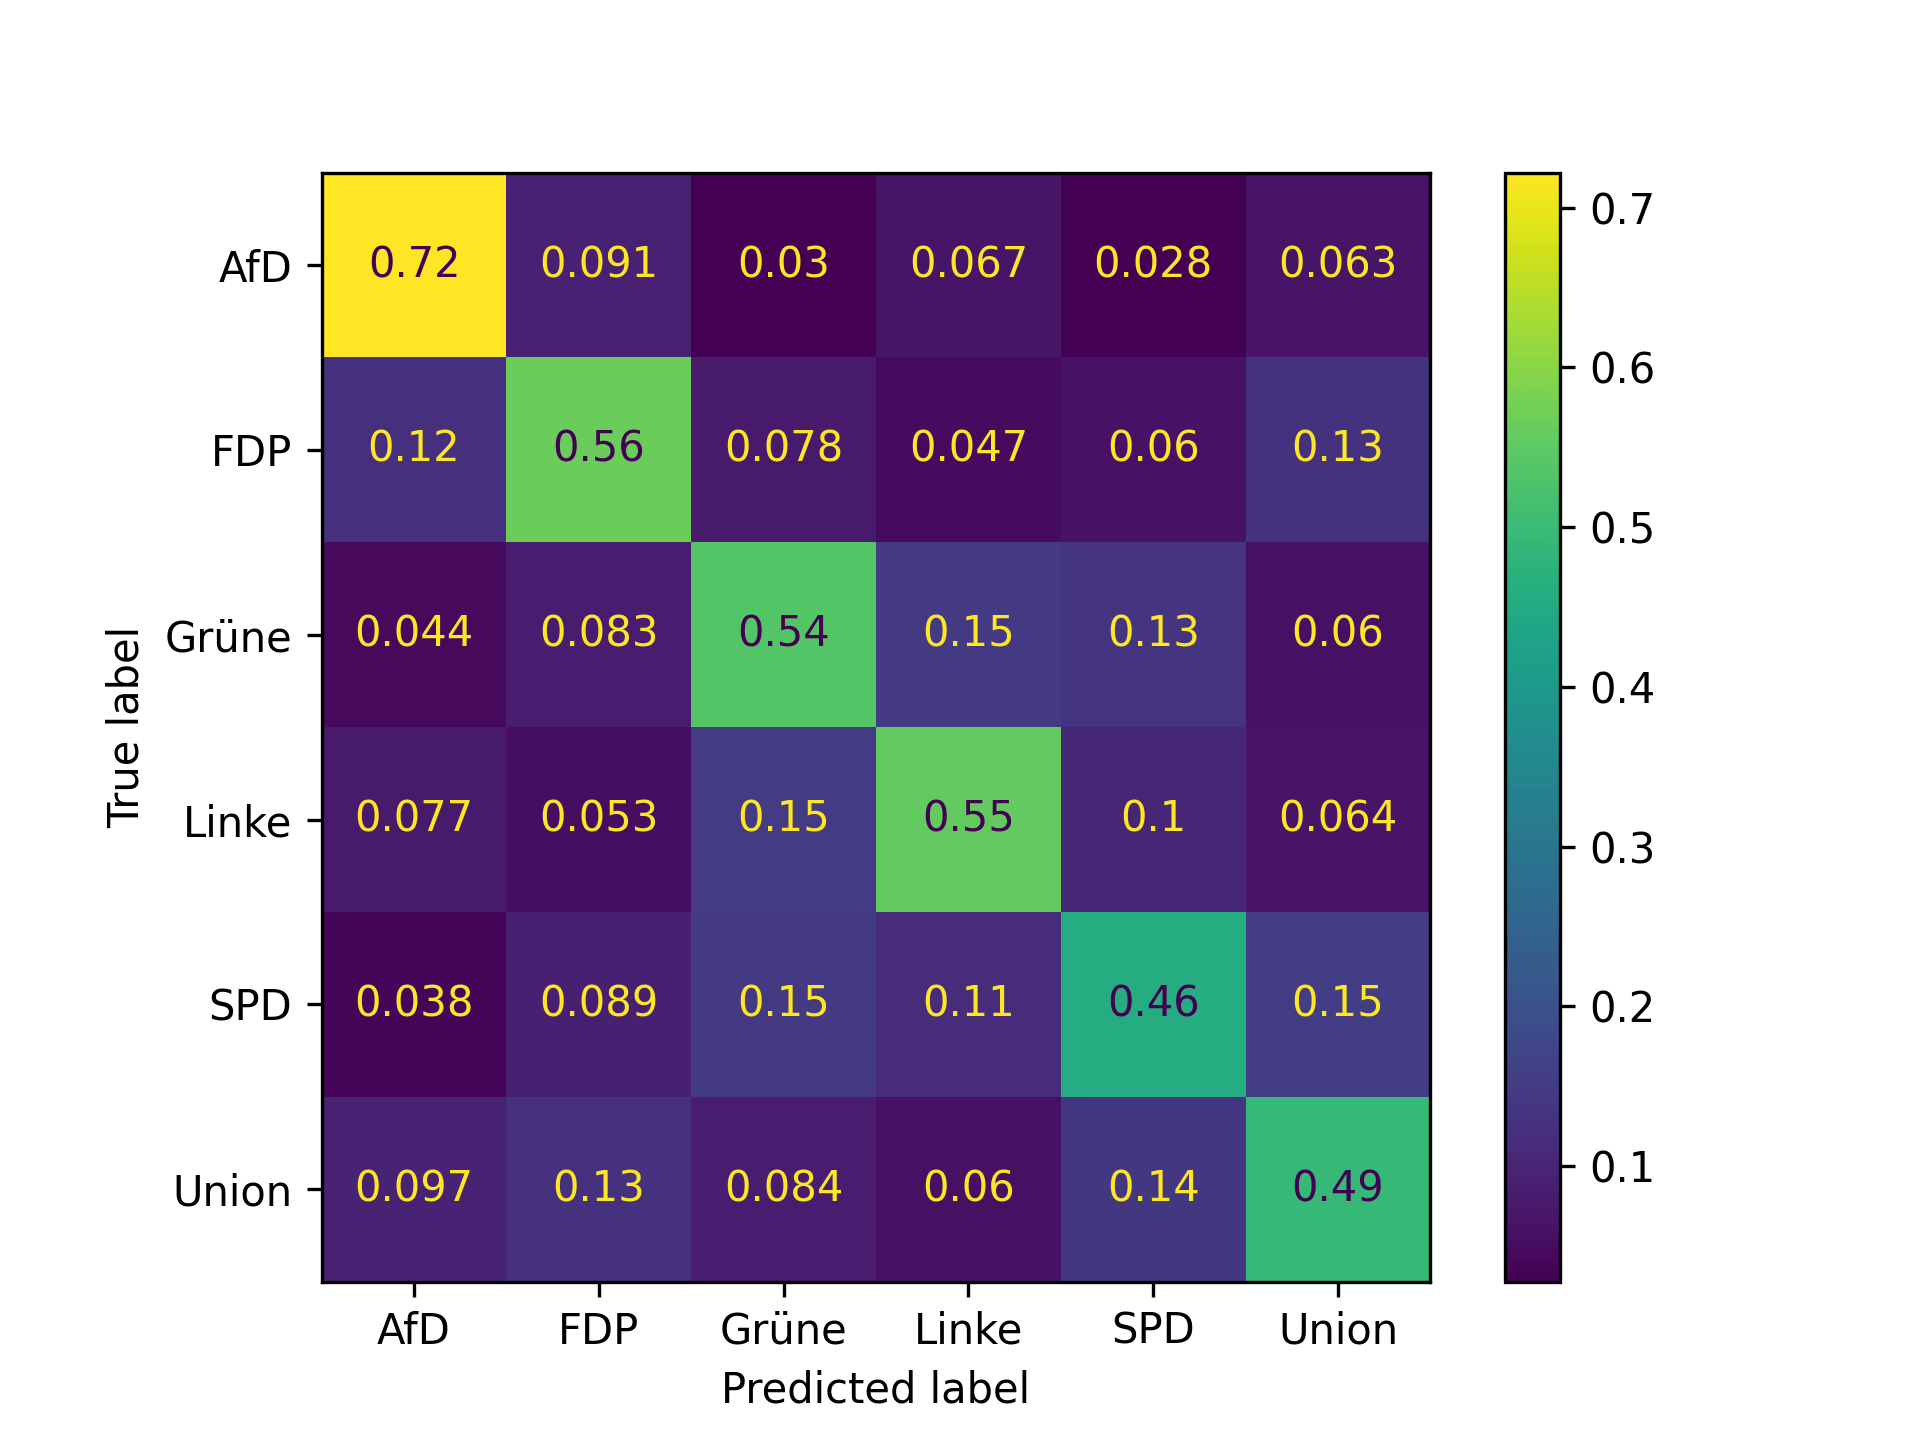
\includegraphics[width=0.9\textwidth]{data/images/modeling/fasttext/under/party_programs_confusion_matrix.png}
      \caption{Wahlprogramme (balanciert, \(N = \num{17949}\))} \label{sfig:confusionMatrixFastTextManifestBalanced}
    \end{subfigure}
    
    \begin{subfigure}{0.5\textwidth}
      \centering
      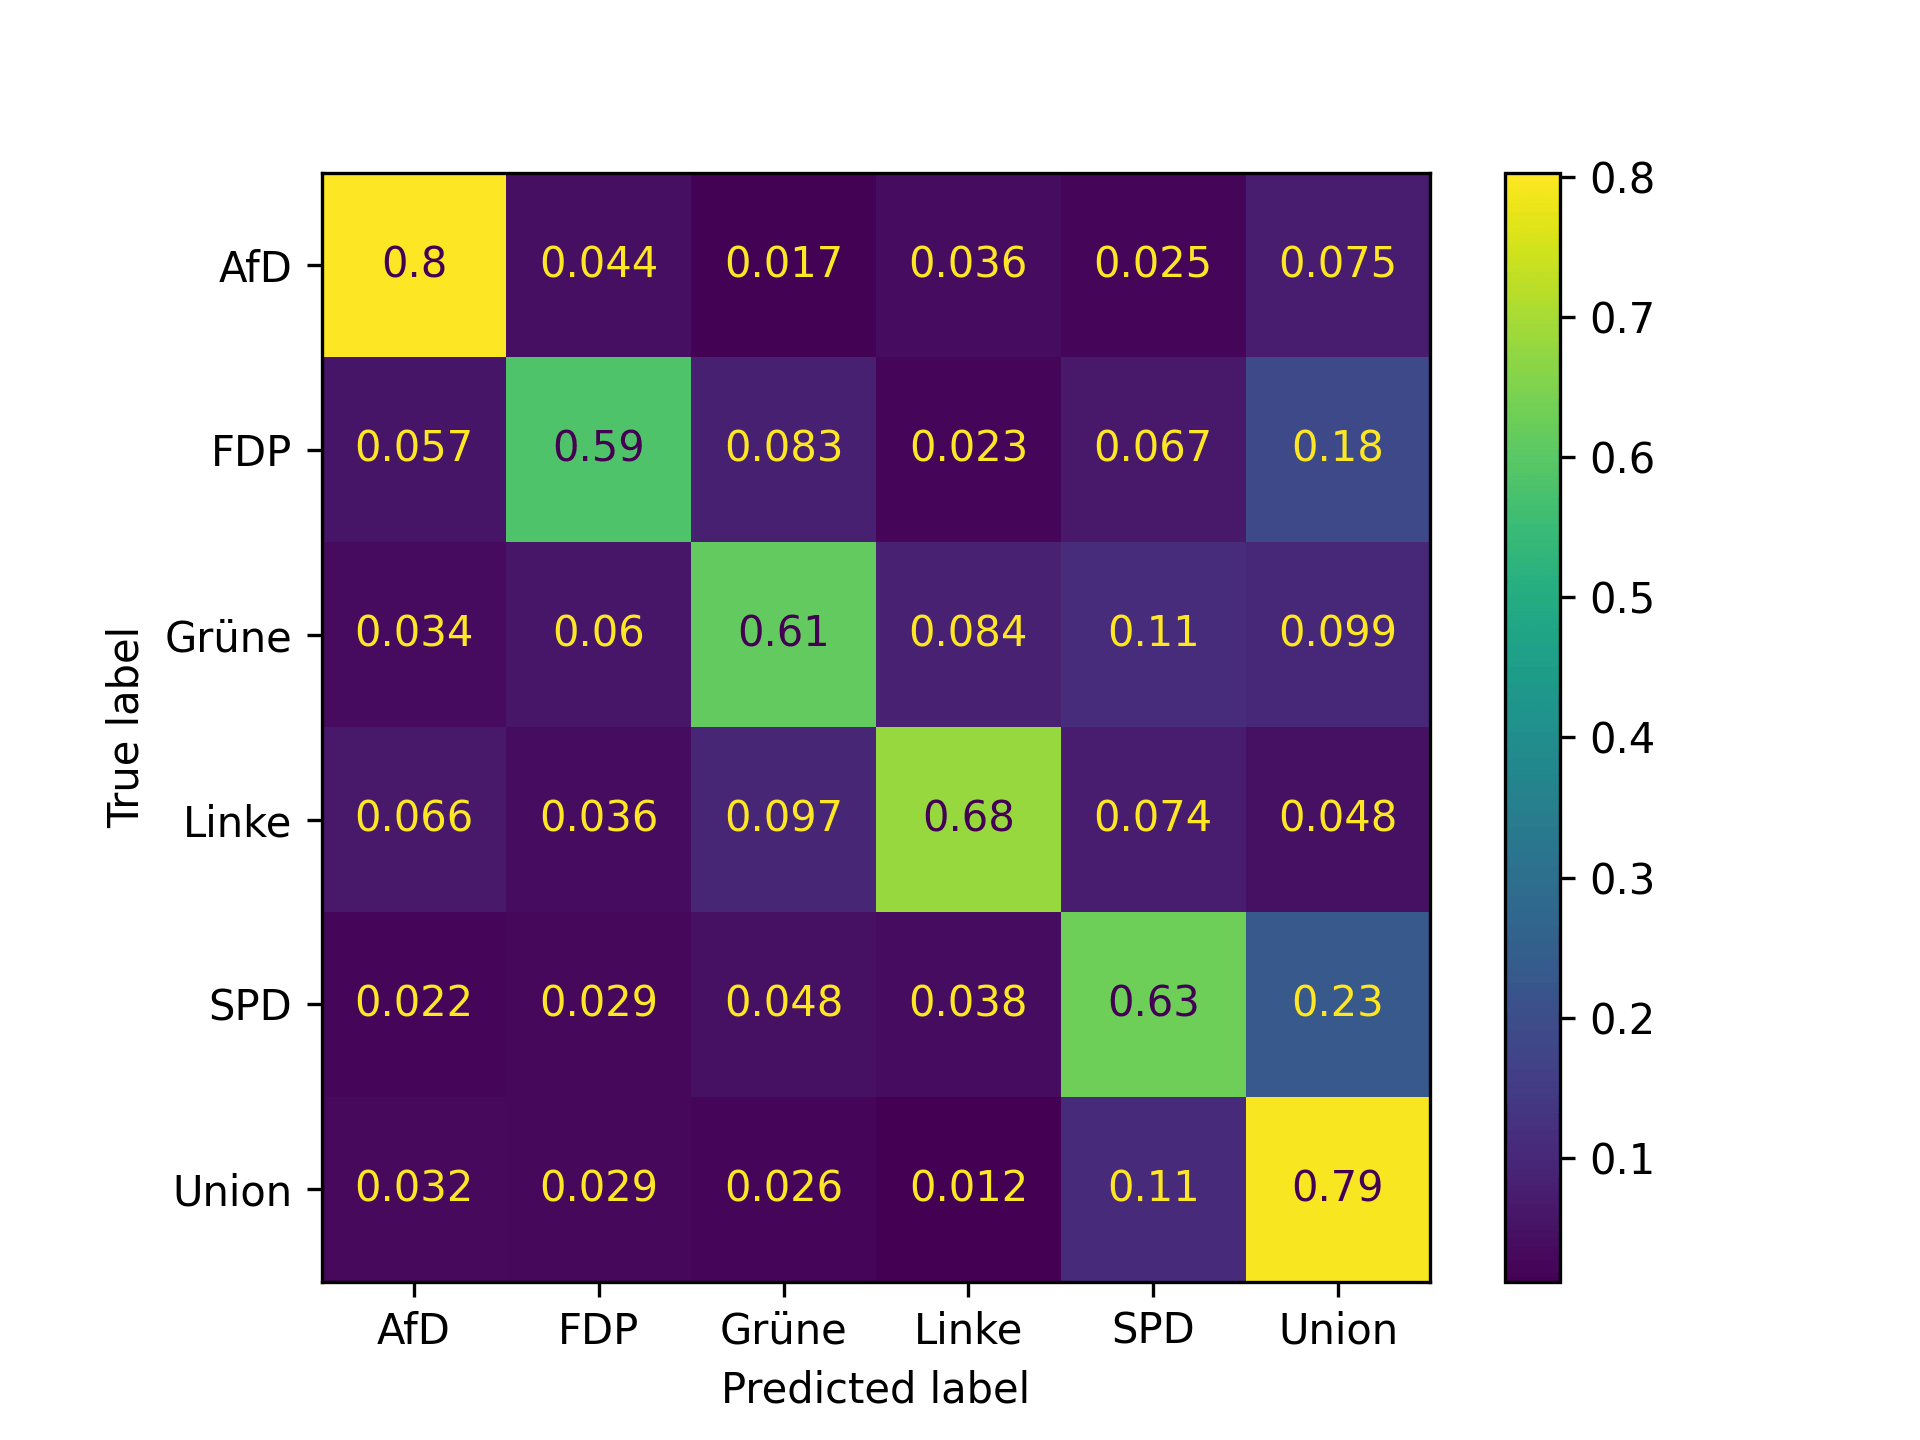
\includegraphics[width=0.9\textwidth]{data/images/modeling/fasttext/none/speeches_confusion_matrix.png}
      \caption{Reden (unbalanciert, \(N = \num{38475}\))} \label{sfig:confusionMatrixFastTextSpeeches}
    \end{subfigure}
    \begin{subfigure}{0.5\textwidth}
      \centering
      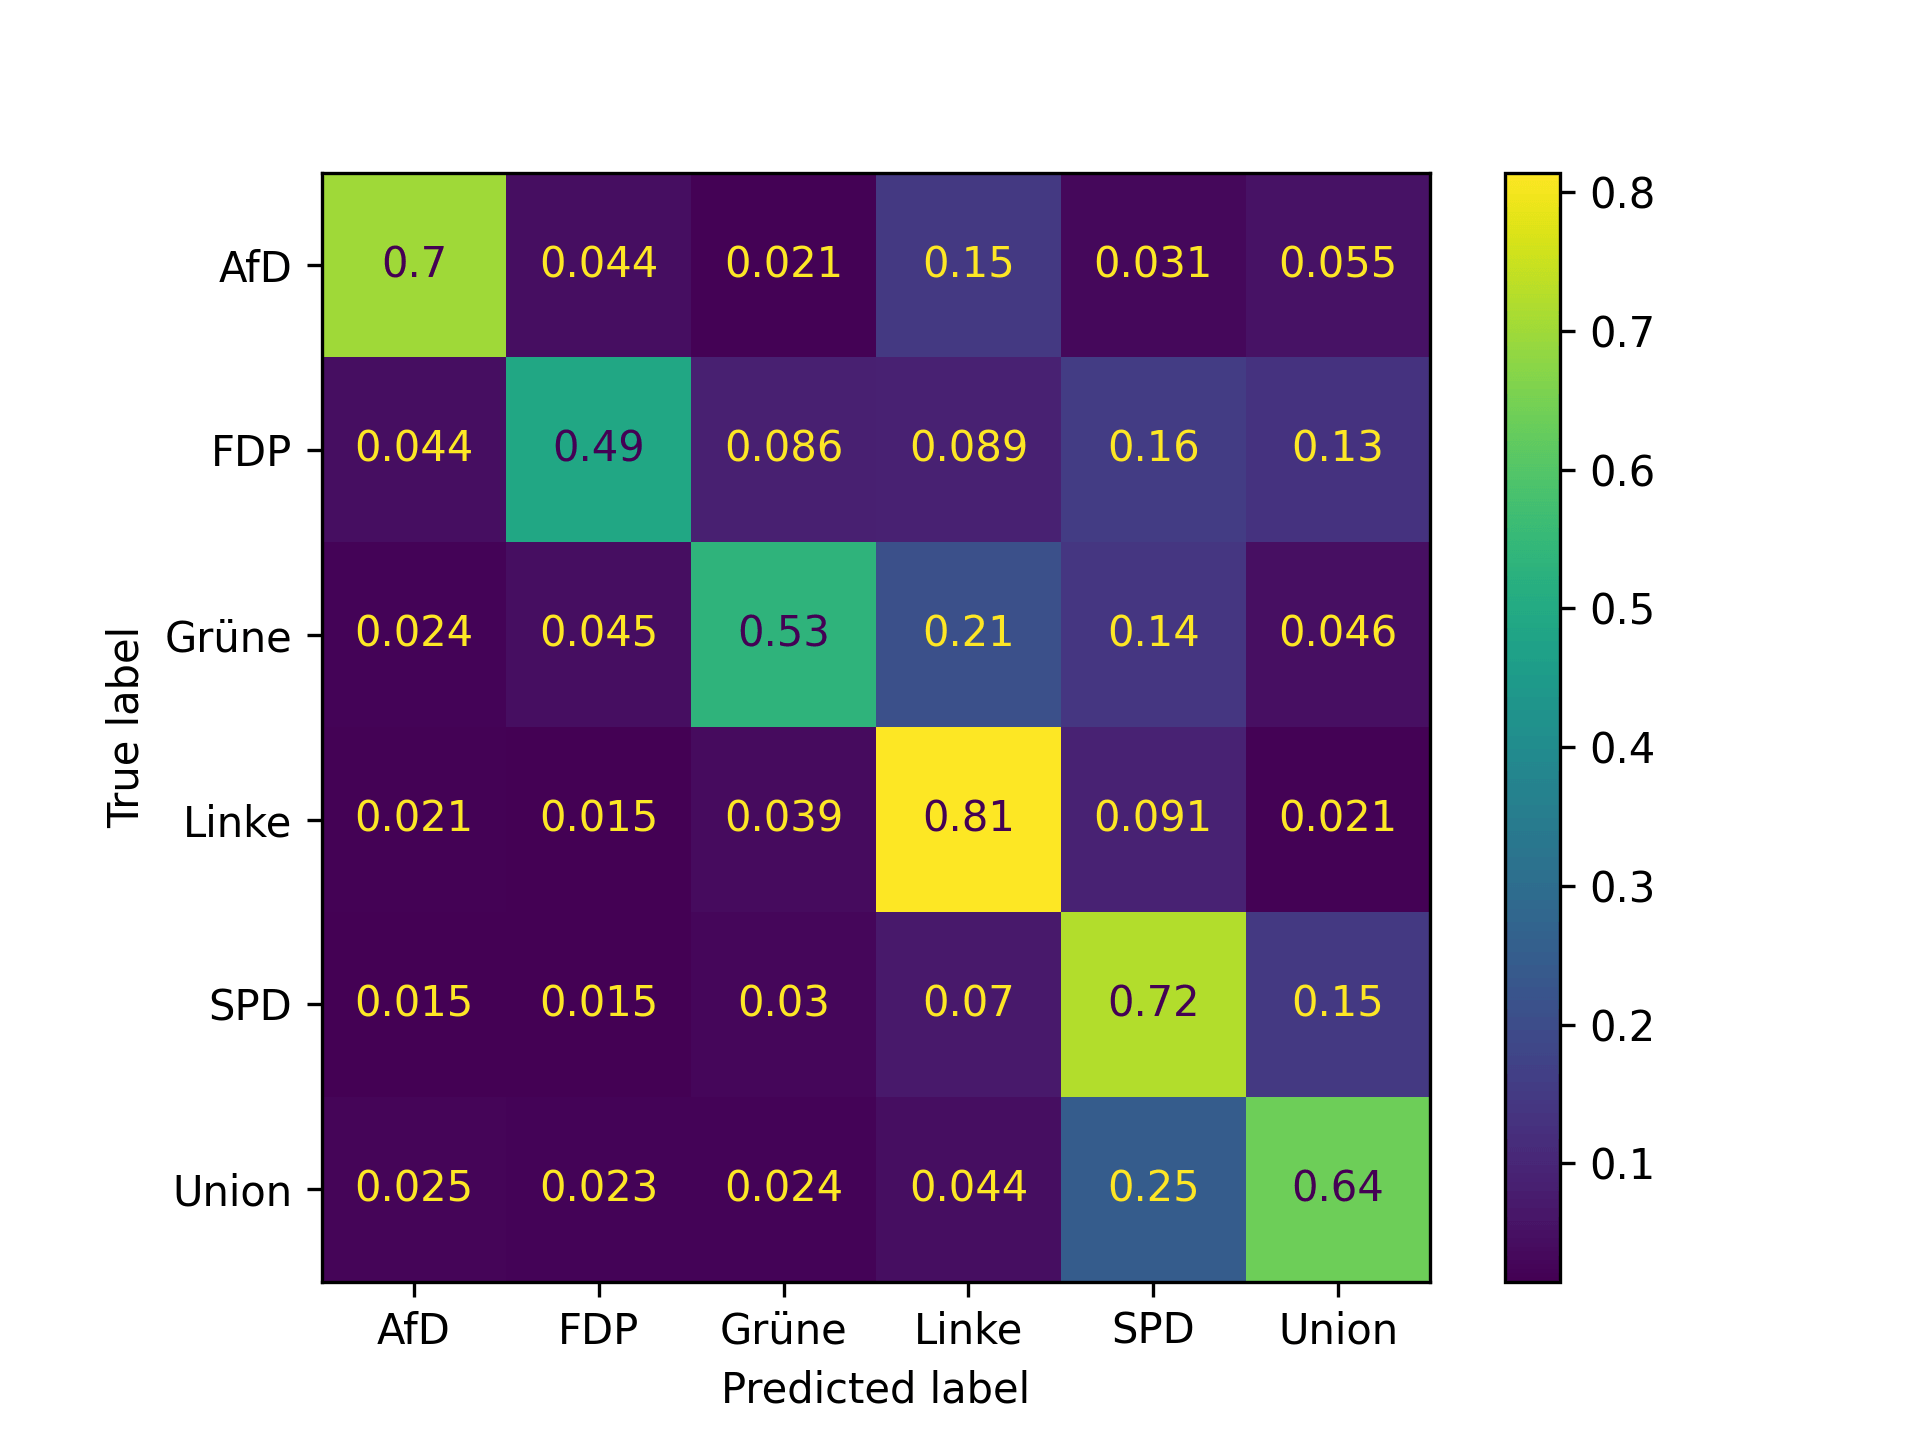
\includegraphics[width=0.9\textwidth]{data/images/modeling/fasttext/under/speeches_confusion_matrix.png}
      \caption{Reden (balanciert, \(N = \num{28719}\))} \label{sfig:confusionMatrixFastTextSpeechesBalanced}
    \end{subfigure}
    
    \caption[Konfusion Matritzen für \ft auf unausgeglichen und ausgeglichenen Datensätzen]{Konfusion Matritzen für \ft auf unausgeglichen und ausgeglichenen Datensätzen und Bigrammen. \(N\) repräsentiert die Anzahl an Trainings- und Testdaten.} \label{fig:confusionMatrixFastText}
\end{figure}

\begin{itemize}
    \item Parteien, die politisch näher beieinander liegen, lassen sich schlechter klassifizieren
    \item \ft ist sehr anfällig für unbalancierte Datensätze
    \item Regierungsparteien neigen zu hoher False Positive Rate untereinander
    \item False Positive Rate segmentiert sich nach Regierungsparteien und Opposition (besonders bei Reden)
\end{itemize}

\subsection{CNN}

\begin{table}[H]
    \centering
    \caption{Scores für Baseline Modelle auf Basis von \acs{BoW} und \acs{TF-IDF}} \label{tab:overviewScoresCNN}
    {\footnotesize
    \begin{tblr}{width=\textwidth, hline{1-2, Z} = {1pt}, row{1}={font=\bfseries}, column{1}={font=\bfseries}}
        Modell & Datensatz & Precision & Recall & \(F_1\) Score \\ 

        SVM + \acs{BoW} & Tweets & \num{0.59} & \num{0.59} & \num{0.59} \\
        SVM + \acs{BoW} & Wahlpro\-gramme & \num{0} & \num{0} & \num{0} \\
        SVM + \acs{BoW} & Reden & \num{0} & \num{0} & \num{0} \\
        \hline
        Lineare Regression + \acs{BoW} & Tweets & \num{0.59} & \num{0.59} & \num{0.59} \\
        Lineare Regression + \acs{BoW} & Wahlpro\-gramme & \num{0} & \num{0} & \num{0} \\
        Lineare Regression + \acs{BoW} & Reden & \num{0} & \num{0} & \num{0} \\
    \end{tblr}
    }
\end{table}

\subsection{BERT}

\section{Out-of-domain}

% TODO: Test specific domain (Textsorten) model with other data (apply tweets to speeches model; out-of-domain) \autocite{biessmann_predicting_2016}

\section{Evaluation} \label{sec:evaluation}

\begin{table}[H]
    \centering
    \caption{Performance von textsortenspezifischen Modellen auf alternativen Testdaten} \label{tab:comparisonModelDatasets}
    {\footnotesize
    \begin{tblr}{width=\textwidth, hline{1-2, Z} = {1pt}, row{1}={font=\bfseries}}
        Datensatz & Tweets & Wahlpro\-gramme & Reden \\ 

        Tweets & N/A & \num{0} & \num{0} \\
        Wahlpro\-gramme & \num{0} & N/A & \num{0} \\
        Reden & \num{0} & \num{0} & N/A \\
    \end{tblr}
    }
\end{table}

% TODO: Update scores and maybe add more models

\begin{table}[H]
    \centering
    \caption{Vergleich des \(F_1\) Scores zwischen \ft und \acs{BERT}} \label{tab:comparisonModels}
    {\footnotesize
    \begin{tblr}{width=\textwidth, hline{1-2, Y-Z} = {1pt}, colspec={l*{3}{Q[si={table-format=1.2},c]}}, row{1}={guard,font=\bfseries,l}, row{5}={font=\bfseries}}
        Datensatz & Precision & Recall & \(F_1\) Score \\ 

        Tweets & 0.59 & 0.59 & 0.59 \\
        Wahlpro\-gramme & 0 & 0 & 0 \\
        Reden & 0 & 0 & 0 \\

        Kombiniert & 0 & 0 & 0 \\
    \end{tblr}
    }
\end{table}

\subsection{Weitere Experimente} \label{subsec:furtherExperiments}

\subsubsection{Alle Daten}

% Alle Tweets (auch Retweets) nutzen und validieren

\subsubsection{Neutrale Klasse}

% 7. Klasse: neutrale Texte (beispielsweise über Wikipedia beziehen)

\subsubsection{Schlussfolgerungen}

% Was sagt unsere Klassifikation am Ende aus? Geht es primär um sprachliche Eigenheiten -- wie Vokabular oder Rhetorik -- oder schließen wir anhand der Themenschwerpunkte auf eine Ideologie?

\subsubsection{Erweiterter Zeitraum}

% Alle Reden (von 1950 bis heute) nutzen und anschließend zeitliche Daten testen

\subsubsection{Betrachtung ausgewählter Klassifikationen}

% Klassifikationsergebnisse von exemplarisch ausgewählten Texten unterschiedlicher Art zwischen mehreren Modellen (die auf anderen Datensätze basieren) vergleichen. Welchen Einfluss haben die verwendeten Daten darauf, was für eine Art von Text jeweils einer Partei besonders stark zugeordnet oder als neutral eingeordnet wird?

\subsubsection{Sentence Level}

% Modelle auf Sentence Level trainiernen

\subsection{Limitationen}

\subsubsection{Feature Engineering}

% TODO: Add example for polysemy

Durch Methoden wie \ac{BoW} und \ac{TF-IDF} gehen syntaktische, als auch semantische Zusammenhänge verloren \autocite[48\psq]{kowsari_text_2019}. Das führt dazu, dass Modelle wie \ac{SVM} und Random Forest ausschließlich die verwendeten Wörter und deren Anzahl in Betracht zieht, aber nicht die tiefere Bedeutung im Kontext des Satzes. Nach \textcite{kowsari_text_2019} versuchen Modelle wie Word2Vec, GloVe und \ft zumindest syntaktische und semantische Zusammenhänge zu berücksichtigen, jedoch haben selbst diese Modelle Schwierigkeiten, Polysemie\footnote{Sätze mit mehreren Bedeutungen} zu klassifizieren.

\subsubsection{Neutralität von Texten} % Sprache, Anzahl an Klassen und fehlende neutrale Klasse

% TODO: Add sources and examples

Des Weiteren ergibt sich aus der Wahl der Datenquellen (Wahlprogramme, Reden und Tweets) eine Annahme/Voraussetzung/Bias geben über der verwendeten Sprache. Wahlprogramme, Reden und Tweets von Politikern weisen zwar parteispezifische Wörter auf, jedoch ist die semantische und syntaktische Komplexität der Sätze überdurchschnittlich hoch. Ebenfalls ist die Menge an Rechtschreibfehlern und verwendetem Slang geringer als bei anderen Textarten. Daraus folgt, dass die Performance der trainierten Modelle voraussichtlich signifikant schlechter ist, wenn Texte sprachlich (semantisch und syntaktisch) stark von den Trainingsdaten abweichen.

% TODO: Rewrite following

Inmitten dieses Projektes hat sich die Frage aufgetan, ob zusätzlich zu den sechs Klassen (Linke, ..., Union) ebenfalls eine neutrale, bzw. nicht klassifizierbare Klasse hinzugefügt werden sollte. Ähnlich zu der Arbeit von \textcite{guhr_training_2020} wo nicht nur positiver und negativer Sentiment analysiert wird, sondern ebenfalls neutral. Dies hat den Hintergrund, dass es ebenfalls Texte gibt, welche keine eindeutig polarisierende Semantik aufweisen. Der gleiche Gedanke lässt sich ebenfalls auf ein politisches Klassifikationsmodell anwenden. Textquellen wie Wikipedia oder fachliche Artikel weisen womöglich eine neutrale, unpolitische Haltung auf. Eine Klassifikation dieser würde irreführend sein. Ein möglicher Lösungsansatz zur Erweiterung der in \autoref{sec:dataUnderstanding} wäre das Hinzufügen von neuralen Texten wie bei \textcite{guhr_training_2020}.

\subsubsection{Politische Nähe}

% TODO: Add sources and image
% TODO: Reason --> Politisches Viereck (links -- rechts, ...)

Parteien, die ähnliche politische Ideale verfolgen, identische Themenschwerpunkte haben, lassen sich schlechter klassifizieren.

\subsubsection{Vortrainierte Worteinbettungen}

Vortrainierte Worteinbettungen sind auf allgemeinen Texten trainiert. Zwischen dem Wortschatz und der Semantik von Wörtern kann daher eine Diskrepanz vorliegen, die zu schlechteren Ergebnissen führt.

% \section{Fazit} \label{sec:crispConclusion_2}
